%% Generated by Sphinx.
\def\sphinxdocclass{report}
\documentclass[a4paper,12pt,french]{sphinxmanual}
\ifdefined\pdfpxdimen
   \let\sphinxpxdimen\pdfpxdimen\else\newdimen\sphinxpxdimen
\fi \sphinxpxdimen=.75bp\relax

\PassOptionsToPackage{warn}{textcomp}
\usepackage[utf8]{inputenc}
\ifdefined\DeclareUnicodeCharacter
% support both utf8 and utf8x syntaxes
\edef\sphinxdqmaybe{\ifdefined\DeclareUnicodeCharacterAsOptional\string"\fi}
  \DeclareUnicodeCharacter{\sphinxdqmaybe00A0}{\nobreakspace}
  \DeclareUnicodeCharacter{\sphinxdqmaybe2500}{\sphinxunichar{2500}}
  \DeclareUnicodeCharacter{\sphinxdqmaybe2502}{\sphinxunichar{2502}}
  \DeclareUnicodeCharacter{\sphinxdqmaybe2514}{\sphinxunichar{2514}}
  \DeclareUnicodeCharacter{\sphinxdqmaybe251C}{\sphinxunichar{251C}}
  \DeclareUnicodeCharacter{\sphinxdqmaybe2572}{\textbackslash}
\fi
\usepackage{cmap}
\usepackage[T1]{fontenc}
\usepackage{amsmath,amssymb,amstext}
\usepackage[french]{babel}
\usepackage{times}
\usepackage[Sonny]{fncychap}
\ChNameVar{\Large\normalfont\sffamily}
\ChTitleVar{\Large\normalfont\sffamily}
\usepackage{sphinx}
\usepackage{pdfpages}

\fvset{fontsize=\small}
\usepackage{geometry}

% Include hyperref last.
\usepackage{hyperref}
% Fix anchor placement for figures with captions.
\usepackage{hypcap}% it must be loaded after hyperref.
% Set up styles of URL: it should be placed after hyperref.
\urlstyle{same}

\addto\captionsfrench{\renewcommand{\figurename}{Fig.\@ }}
\makeatletter
\def\fnum@figure{\figurename\thefigure{}}
\makeatother
\addto\captionsfrench{\renewcommand{\tablename}{Tableau }}
\makeatletter
\def\fnum@table{\tablename\thetable{}}
\makeatother
\addto\captionsfrench{\renewcommand{\literalblockname}{Code source}}

\addto\captionsfrench{\renewcommand{\literalblockcontinuedname}{suite de la page précédente}}
\addto\captionsfrench{\renewcommand{\literalblockcontinuesname}{suite sur la page suivante}}
\addto\captionsfrench{\renewcommand{\sphinxnonalphabeticalgroupname}{Non-alphabetical}}
\addto\captionsfrench{\renewcommand{\sphinxsymbolsname}{Symboles}}
\addto\captionsfrench{\renewcommand{\sphinxnumbersname}{Numbers}}

\addto\extrasfrench{\def\pageautorefname{page}}

\setcounter{tocdepth}{1}



\title{eyes17 Documentation}
\date{févr. 28, 2020}
\release{1.0}
\author{GK}
\newcommand{\sphinxlogo}{\vbox{}}
\renewcommand{\releasename}{Version}
\makeindex
\begin{document}

\ifdefined\shorthandoff
  \ifnum\catcode`\=\string=\active\shorthandoff{=}\fi
  \ifnum\catcode`\"=\active\shorthandoff{"}\fi
\fi

\pagestyle{empty}

\includepdf{coverpage.pdf}
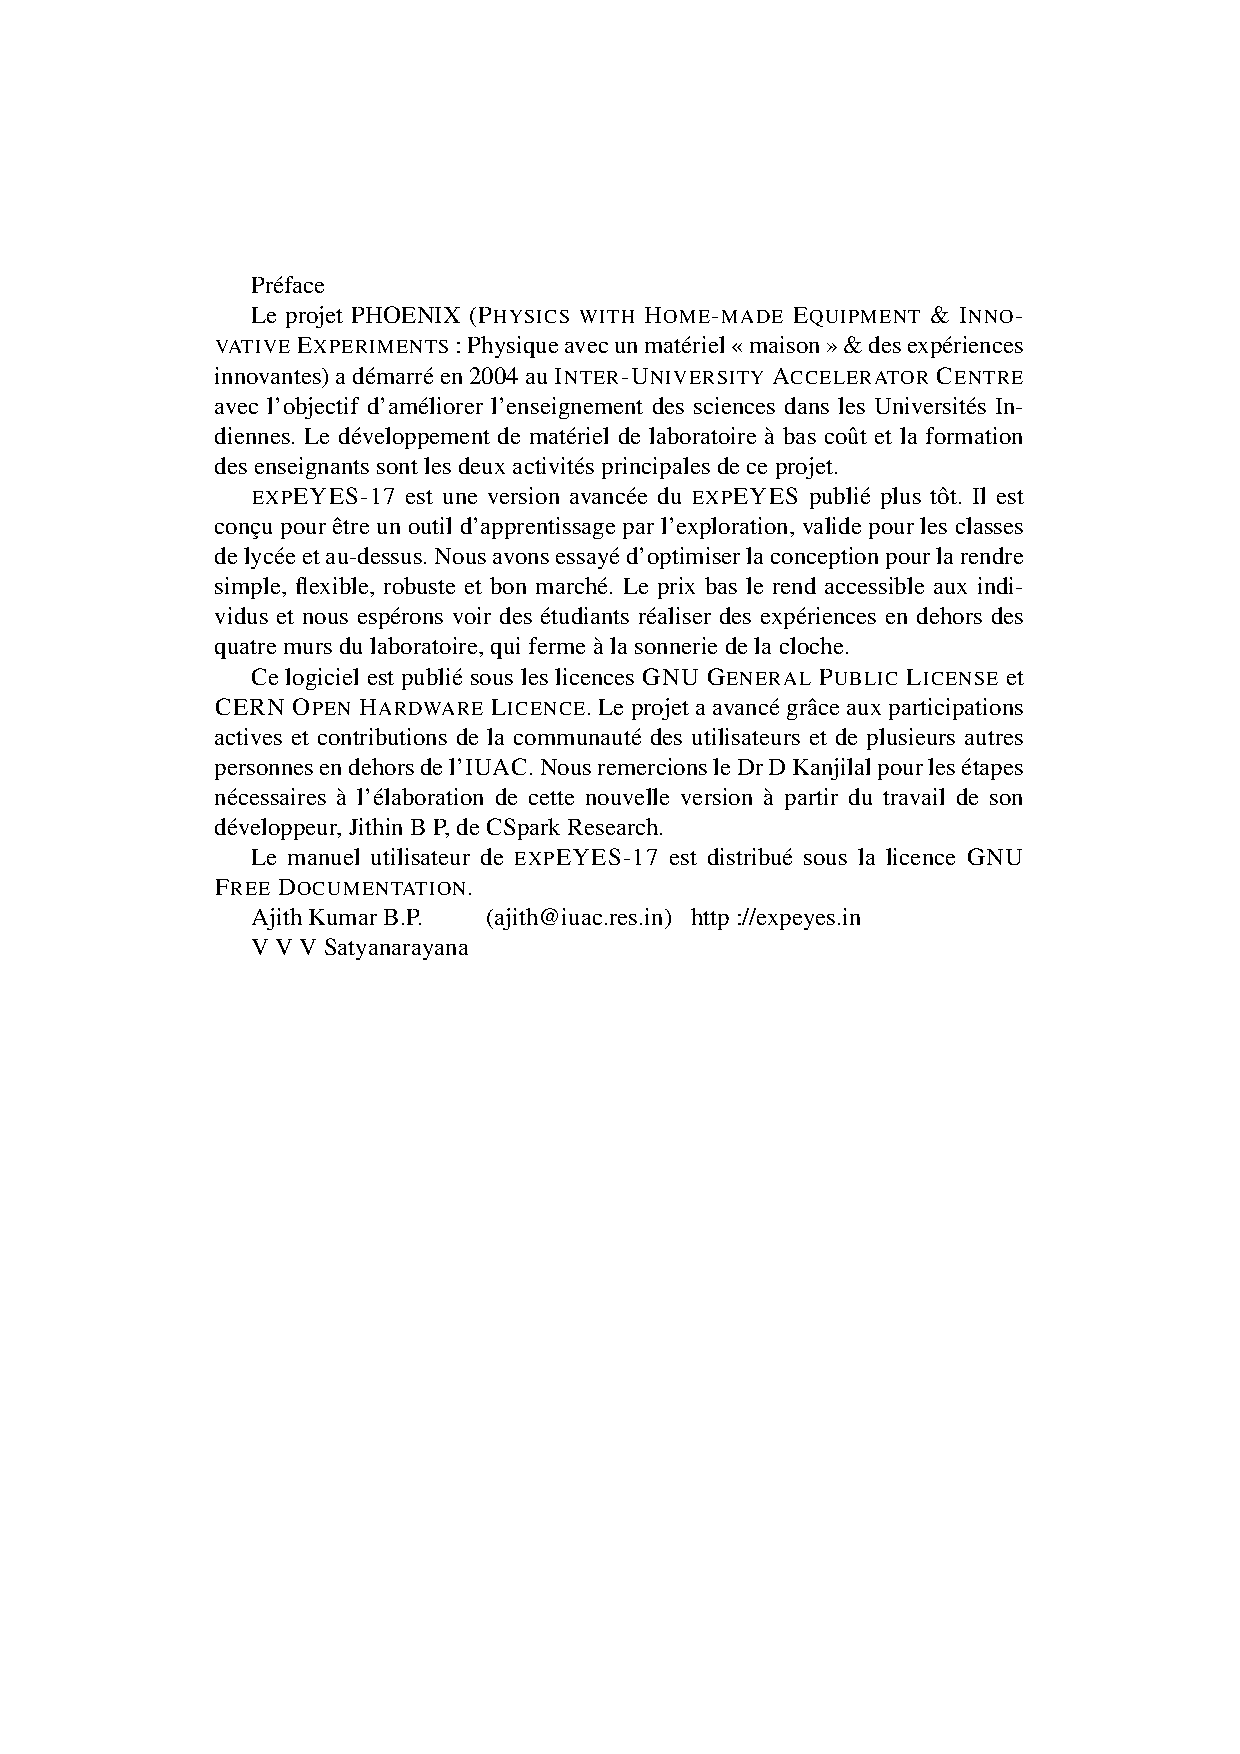
\includepdf{preface.pdf}
\pagestyle{plain}
\sphinxtableofcontents
\pagestyle{normal}
\phantomsection\label{\detokenize{index::doc}}



\chapter{Introduction}
\label{\detokenize{1.1:introduction}}\label{\detokenize{1.1::doc}}
La science est l’étude du monde physique par des observations systématiques
et des expériences. Une bonne éducation scientifique est essentielle
pour cultiver une société où le raisonnement et la pensée logique
prévalent au lieu de la superstition et des croyances irrationnelles.
L’éducation scientifique est aussi essentielle pour former suffisamment
de techniciens, d’ingénieurs et de scientifiques pour l’économie du
monde moderne. On admet largement que l’expérience personnelle issue
d’expérimentations et d’observations réalisées soit par les étudiants,
soit par des enseignants à titre de démonstration, soit essentielle
à la pédagogie de la science. Cependant, presque partout la science
est enseignée en grande partie à partir de livres de cours sans donner
d’importance à l’expérimentation, en partie à cause du manque d’équipements.
Sans surprise, la plupart des étudiants échouent à corréler leurs
connaissance acquise en classe aux problèmes rencontrés dans la vie
quotidienne. On peut jusqu’à un certain point corriger cela en enseignant
la science à l’aide de questionnements et d’expériences.

L’avènement des ordinateurs personnels et leur banalisation a ouvert
une nouvelle voie pour faire des expériences de laboratoire. L’ajout
d’un peu de matériel à un ordinateur ordinaire peut le convertir en
un laboratoire de sciences. Réaliser des mesures rapides avec une
bonne précision autorise l’étude une large palette de phénomènes.
Les expériences scientifiques impliquent en général la mesure et le
contrôle de certains paramètres physiques comme la température, la
pression, la vitesse, l’accélération, la force, la tension, le courant,
etc. Si la grandeur physique étudiée évolue rapidement, il faut automatiser
la mesure et un ordinateur devient utile. Par exemple, comprendre
la variation de la tension alternative du secteur nécessite de la
mesurer à chaque milliseconde.

La possibilité de réaliser des expériences avec une précision raisonnable
ouvre aussi la possibilité d’une éducation scientifique orientée sur
la recherche. Les étudiants peuvent comparer les données expérimentales
avec des modèles mathématiques et examiner les lois fondamentales
qui régissent de nombreux phénomènes. Le kit expEYES ( expEriments
for Young Engineers \& Scientists) est conçu pour permettre une grande
variété d’expériences, de l’école à l’université. Il est aussi utilisable
comme un équipement de test pour des ingénieurs en électronique ou
des bricoleurs. L’architecture simple et ouverte d’expEYES permet
aux utilisateurs de développer de nouvelles expériences, sans rentrer
dans les détails de l’électronique et de la programmation d’ordinateurs.
Ce manuel utilisateur décrit \sphinxstyleemphasis{expEYES-17} avec plusieurs expériences,
et il y a aussi un manuel du programmeur.


\chapter{Le matériel}
\label{\detokenize{1.2:le-materiel}}\label{\detokenize{1.2::doc}}
ExpEYES-17 est interfacé et alimenté grâce au port USB de l’ordinateur.
Pour y connecter des signaux externes, il a plusieurs entrées/sorties,
situées de chaque côté, comme montré sur la figure {\hyperref[\detokenize{1.2:fig-e17}]{\sphinxcrossref{\DUrole{std,std-ref}{ExpEYES17}}}}.
Il peut surveiller et contrôler des tensions à ses connexions. Pour
mesurer d’autres paramètres (tels que la température, la pression,
etc.), on a besoin de les convertir en signaux électriques à l’aide
de capteurs adéquats.

La précision des mesures de tension est conditionnée par la stabilité
de la référence à \(3,3~V\) utilisée, elle varie de \(50~ppm\) par degré
Celsius. Les erreurs de gain et d’offset sont éliminées par une calibration
initiale, à l’aide du convertisseur analogique-numérique 16 bits.

Bien que notre premier objectif soit de faire des expériences, nous
vous conseillons de lire la brève description du matériel ci-dessous.
L’appareil peut être aussi utilisé comme matériel de test pour des
expériences d’électricité et d’électronique.

\sphinxstylestrong{IMPORTANT :}

\sphinxstyleemphasis{Les tensions extérieures connectées à ExpEYES17 doivent être comprises dans les limites autorisées. Les entrées A1 et A2 doivent être dans l’intervalle}
\(\pm16\)
\sphinxstyleemphasis{volts et les entrées IN1 and IN2 doivent être dans l’intervalle de 0 à 3,3 V. Des tension excessives peuvent provoquer des dommages permanents. Pour mesurer des tensions plus hautes, diminuez-les en utilisant des diviseurs de tensions.}

\begin{figure}[htbp]
\centering
\capstart

\noindent\sphinxincludegraphics[width=500\sphinxpxdimen]{{eyes17-panel}.pdf}
\caption{ExpEYES17}\label{\detokenize{1.2:id1}}\label{\detokenize{1.2:fig-e17}}
\begin{sphinxlegend}
La face avant d’ExpEYES17 avec les connexions externes sur le dessus.
\end{sphinxlegend}
\end{figure}


\section{Connexions externes}
\label{\detokenize{1.2:connexions-externes}}
Les fonctions des connexions externes sont expliquées brièvement ci-dessous.
Toutes les bornes de couleur noire sont des masses (0 V), toutes
les autres tensions sont mesurées par rapport à elles.


\subsection{Les sorties :}
\label{\detokenize{1.2:les-sorties}}

\subsubsection{Source de courant constant (CCS) :}
\label{\detokenize{1.2:source-de-courant-constant-ccs}}
La source de courant constant peut être activée ou désactivée (ON
et OFF) sous contrôle logiciel.La valeur nominale est 1,1 mA mais
peut varier d’une unité à l’autre, à cause de la tolérance des composants.
Pour mesurer sa valeur exacte, connecter un ampèremètre entre CCS
et GND. Une autre méthode consiste à connecter une résistance connue
(environ \(1~k\Omega\)) et mesurer la différence de potentiel
à ses bornes. La résistance de charge doit être inférieure à \(3~k\Omega\)
pour cette source de courant.


\subsection{Tension programmable (PV1) :}
\label{\detokenize{1.2:tension-programmable-pv1}}
Elle peut être réglée, par logiciel, à toute valeur comprise dans
l’intervalle de -5 V à +5 V. La résolution est 12 bits, ce qui implique
une résolution en tension d’environ \(2,5~mV\).


\subsubsection{Tension programmable (PV2) :}
\label{\detokenize{1.2:tension-programmable-pv2}}
Elle peut être réglée, par logiciel, à toute valeur comprise dans
l’intervalle de -3,3 V à +3,3 V. La résolution est 12 bits.


\subsubsection{Signal carré SQ1:}
\label{\detokenize{1.2:signal-carre-sq1}}
La sortie oscille entre 0 et 5 V et la fréquence peut être ajustée
entre 10 Hz et 100 kHz. Toutes les valeurs intermédiaires de fréquence
ne sont pas possibles. On peut programmer le rapport cyclique. Quand
on règle la fréquence à 0 Hz provoque un état HAUT à la sortie, et
si on la règle à -1 Hz, la sortie passe à l’état BAS ; dans les
deux cas la génération de signal carré est désactivée. La sortie SQR1
comporte une \sphinxstylestrong{résistance série} de \(100~\Omega\)
intégrée si bien qu’elle peut commander des DELs directement.


\subsubsection{Signal carré SQ2:}
\label{\detokenize{1.2:signal-carre-sq2}}
La sortie oscille entre 0 et 5 V et la fréquence peut être ajustée
entre 10 Hz et 100 kHz. Toutes les valeurs intermédiaires de fréquence
ne sont pas possibles. On peut programmer le rapport cyclique. La
sortie SQR2 n’est pas disponible quand on active WG.


\subsubsection{Sortie numérique (OD1) :}
\label{\detokenize{1.2:sortie-numerique-od1}}
La tension en OD1 peut être réglée à 0 ou 5 V, par logiciel.


\subsubsection{Signal Sinusoïdal/Triangulaire WG :}
\label{\detokenize{1.2:signal-sinusoidal-triangulaire-wg}}
Sa fréquence peut être ajustée entre 5 Hz et 5 kHz. La valeur crête
peut être réglées à 3 V, 1,0 V ou 80 mV. La forme du signal est
programmable. À l’aide de l’interface utilisateur on peut sélectionner
une forme sinusoïdale ou triangulaire. \(\overline{WG}\) est le signal
de WG, inversé..


\subsection{Entrées :}
\label{\detokenize{1.2:entrees}}

\subsubsection{Mesure de capacité en IN1 :}
\label{\detokenize{1.2:mesure-de-capacite-en-in1}}
On peut mesurer la valeur d’un condensateur connecté entre IN1 et
GND. Ça marche mieux pour de petites valeurs de capacité, jusqu’à
10 nF, les résultats sont moins précis au-delà.


\subsubsection{Fréquencemètre en IN2 :}
\label{\detokenize{1.2:frequencemetre-en-in2}}
Celui-ci est capable de mesurer des fréquences jusqu’à plusieurs MHz.


\subsubsection{Capteur de résistance (SEN) :}
\label{\detokenize{1.2:capteur-de-resistance-sen}}
Cette entrée est surtout conçue pour des capteurs comme des photorésistances
(LDR), des thermistances, des photo-transistors, etc. L’entrée SEN
est connectée en interne à 3,3 V à travers une résistance de \(5,1~k\Omega\).


\subsubsection{Entrées analogiques:math:\sphinxtitleref{pm16V}, A1 \& A2 :}
\label{\detokenize{1.2:entrees-analogiques-math-pm16v-a1-a2}}
Celles-ci peuvent mesurer des tensions dans l’intervalle \(\pm16~V\).
On peut choisir le calibre de 0,5 V à 16 V en pleine échelle. On
peut visualiser la tension de ces entrées en fonction du temps, ce
qui donne une fonction d’oscilloscope pour basses fréquences. La plus
grande vitesse d’échantillonnage est 1 Méch/s pour un seul canal.
Chacune des entrées a une impédance de \(1~M\Omega\) .


\subsubsection{Entrée analogique \protect\(\pm3.3V\protect\) A3 :}
\label{\detokenize{1.2:entree-analogique-pm3-3v-a3}}
Celle-ci peut mesurer une tension dans l’intervalle \(\pm3.3~V\). On
peut amplifier cette entrée en connectant une résistance entre Rg
et GND, gain = \(1+\frac{Rg}{10000}\). Cela permet d’afficher des signaux
de très petite amplitude. L’impédance de l’entrée A3 est \(10~M\Omega\).


\subsubsection{Entrée Microphone MIC :}
\label{\detokenize{1.2:entree-microphone-mic}}
Un microphone à condensateur peut être connecté à cette borne afin
de capturer le signal à la sortie.


\subsection{Interface pour les capteurs I2C :}
\label{\detokenize{1.2:interface-pour-les-capteurs-i2c}}
Les quatre connexions (+5 V, GND, SCL et SDA) situées sur la bande
de connexions Berg supporte les capteurs de la famille I2C. Le logiciel
peut reconnaître un grand nombre de capteurs I2C disponibles dans
le commerce.


\subsection{Alimentation \protect\(\pm6~V/10~mA\protect\)  :}
\label{\detokenize{1.2:alimentation-pm6-v-10-ma}}
Les bornes VR+ et VR- sont des alimentations régulées. Elles fournissent
peut de courant, mais assez pour alimenter un ampli-op.


\section{Kit d’accessoires}
\label{\detokenize{1.2:kit-d-accessoires}}
Quelques accessoires sont livrés avec expEYES.
\begin{itemize}
\item {} 
Fils électriques, avec une borne rigide mâle et avec une pince crocodile.

\item {} 
Microphone à condensateur avec ses fils.

\item {} 
Bobine d’induction (2) : du fil isolé 44SWG enroulé dans une bobine
de diamètre 1 cm. Environ 3000 tours (il peut y avoir quelques tours
de plus). On peut utiliser ces bobines pour étudier l’inductance,
l’induction électromagnétique, etc.

\item {} 
Disque piézo-électrique (2) : sa fréquence de résonance est d’environ
3500 Hz. Il peut être alimenté par la sortie WG ou SQR1. Le disque
est enfermé dans une coquille en plastique formant une cavité, qui
augmente l’amplitude du son produit.

\item {} 
Moteur CC : doit être alimenté par une tension continue de moins
de 3 V.

\item {} 
Aimants permanents : (a) diamètre et longueur 10 mm (b) diamètre
5 mm et longueur 10 mm (c) aimants de taille bouton(2)

\item {} 
DELs 5 mm : rouge, bleue, verte, blanche.

\item {} 
Condensateurs : 100 pF, 0.1 µF , 1 µF et 22 µF

\item {} 
Inductances : 10 mH / \(20~\Omega\),

\item {} 
Résistances :
\(560~\Omega\), \(1~k\Omega\), \(2,2~k\Omega\) ,
\(10~k\Omega\),
\(51~k\Omega\) et \(100~k\Omega\)

\item {} 
photorésistance (LDR )

\item {} 
Deux diodes silicium (\sphinxcode{\sphinxupquote{1N4148}}) et une diode Zéner de \(3,3~V\)

\item {} 
Transistor NPN (\sphinxcode{\sphinxupquote{2N2222}})

\end{itemize}


\chapter{Installation du logiciel}
\label{\detokenize{1.3:installation-du-logiciel}}\label{\detokenize{1.3::doc}}
ExpEYES peut fonctionner sur tout ordinateur disposant d’un interpréteur
Python et d’un module Python pour accéder au port série. L’interface
USB est prise en charge par le programme pilote qui présente le port
USB comme un port RS232 aux programmes d’applications. La communication
avec le boîtier expEYES est réalisée à l’aide d’une bibliothèque écrite
en langage Python.

Des programmes avec une interface utilisateur graphique ont été écrits
pour de nombreuses expériences. Le logiciel Eyes17 dépend des paquets
logiciels suivants :
\begin{itemize}
\item {} 
\sphinxcode{\sphinxupquote{python3-serial}}

\item {} 
\sphinxcode{\sphinxupquote{python3-numpy}}

\item {} 
\sphinxcode{\sphinxupquote{python3-scipy}}

\item {} 
\sphinxcode{\sphinxupquote{python3-qt5}}

\item {} 
\sphinxcode{\sphinxupquote{python3-pyqtgraph}}

\end{itemize}


\section{Pour toute distribution GNU/Linux :}
\label{\detokenize{1.3:pour-toute-distribution-gnu-linux}}
Télécharger \sphinxstylestrong{eyes17-x.x.x.zip} (la dernière version) depuis
\sphinxstylestrong{http://expeyes.in} et dézipper ce fichier, puis aller dans
le nouveau dossier. Taper les commandes :

\begin{sphinxVerbatim}[commandchars=\\\{\}]
\PYGZdl{} sudo sh postinst       \PYGZsh{} donne la permission d\PYGZsq{}accès à tous

\PYGZdl{} python main.py
\end{sphinxVerbatim}

Vous aurez des messages d’erreur pour tout paquet manquant qui pourrait
être nécessaire à expeyes. Installer ces paquets et réessayer. Les
programmes Python nécessaires pour de nombreuses expériences sont
dans le même répertoire, ils sont appelés par \sphinxcode{\sphinxupquote{main.py}}.


\section{Distributions GNU/Linux Debian ou Ubuntu}
\label{\detokenize{1.3:distributions-gnu-linux-debian-ou-ubuntu}}
Télécharger \sphinxstylestrong{eyes17-x.x.x.deb} (la dernière version) depuis
la zone de téléchargement de \sphinxstylestrong{http://expeyes.in} et l’installer
à l’aide de la commande :

\begin{sphinxVerbatim}[commandchars=\\\{\}]
\PYGZdl{} sudo gdebi eyes17\PYGZhy{}x.x.x.deb
\end{sphinxVerbatim}

alors qu’on est connecté à Internet

Le paquet \sphinxcode{\sphinxupquote{eyes17}} (de version supérieure à 3) ne dépend
pas de versions antérieures d’ExpEYES, comme expeyes-junior. Pendant
l’installation \sphinxcode{\sphinxupquote{gdebi}} téléchargera automatiquement et installera
les paquets requis.

\sphinxstylestrong{N.B. :} on peut aussi utiliser la commande :

\begin{sphinxVerbatim}[commandchars=\\\{\}]
\PYGZdl{} sudo apt install eyes17
\end{sphinxVerbatim}

alors qu’on est connecté à Internet ; le paquet \sphinxcode{\sphinxupquote{eyes17}} disponible
dans la distribution (actuellement dans debian/buster ou ubuntu/bionic)
ainsi que toutes ses dépendances sera téléchargé et installé.


\section{Le CD vif expEYES / La clé USB vive}
\label{\detokenize{1.3:le-cd-vif-expeyes-la-cle-usb-vive}}
L’image ISO qui offre le support pour eyes17 est disponible ICI pour
téléchargement. Créer un DVD ou une clé USB démarrables à l’aide cette
image ISO (télécharger rufus depuis \sphinxurl{https://rufus.akeo.ie} pour faire
ça sous MSWindows)

Éteindre le PC et brancher la clé USB ou insérer le CD vif, puis démarrer
l’ordinateur. Entrer dans le BIOS durant la phase de démarrage, et
faire en sorte que le CD ou la clé USB soit prise en compte comme
premier média de démarrage. Redémarrer en enregistrant ce réglage.
Un bureau apparaîtra et on peut lancer expEYES-17 depuis le menu \sphinxstylestrong{Applications-\textgreater{}Éducation}-\textgreater{}ExpEYES-17.

On peut aussi le lancer depuis un terminal à l’aide de la commande :

\begin{sphinxVerbatim}[commandchars=\\\{\}]
\PYGZdl{} python /usr/share/expeyes/eyes17/main.py
\end{sphinxVerbatim}


\section{Sous MSWindows}
\label{\detokenize{1.3:sous-mswindows}}
Il faut tout d’abord installer le logiciel pilote pour le convertisseur
USB Série MCP2200, disponible sur le site de Microchip (et aussi disponible
sur le site expeyes). Après installation de ce pilote apparaîtra un
port COM, qu’on peut tester à l’aide du gestionnaire de périphériques
de MSWindows. Ensuite il y a deux options.

Un fichier zip contenant toutes les choses nécessaires pour ExpEYES
est disponible sur le site expeyes, sous le nom \sphinxcode{\sphinxupquote{eyes17win.zip}}.
Télécharger et dézipper ce fichier puis lancer \sphinxcode{\sphinxupquote{main.py}}
à partir de là. En utilisant cette méthode, on ne pourra pas écrire
soi-même de code Python pour accéder à expeyes ; pour ce faire il
faut installer comme suit :
\begin{itemize}
\item {} 
\sphinxcode{\sphinxupquote{Python version 2.x}}

\item {} 
\sphinxcode{\sphinxupquote{python-serial}}

\item {} 
\sphinxcode{\sphinxupquote{python-qt4}}

\item {} 
\sphinxcode{\sphinxupquote{python-pyqtgraph}}

\item {} 
\sphinxcode{\sphinxupquote{python-numpy}}

\item {} 
\sphinxcode{\sphinxupquote{python-scipy}}

\end{itemize}

Télécharger le fichier \sphinxcode{\sphinxupquote{eyes17-x.x.x.zip}} (la dernière version)
depuis le site web. En dézippant ce fichier on obtient un dossier
nommé \sphinxcode{\sphinxupquote{**eyes17**}}, lancer \sphinxcode{\sphinxupquote{**main.py**}}
depuis là.


\chapter{Le programme graphique principal}
\label{\detokenize{1.4:le-programme-graphique-principal}}\label{\detokenize{1.4::doc}}
Démarrer Applications-\textgreater{}Éducation-\textgreater{}ExpEYES-17 depuis le menu. Un écran
d’oscilloscope à quatre canaux avec de nombreuses fonctionnalités
en plus, s’ouvrir comme affiché sur la figure {\hyperref[\detokenize{1.4:the-scope17-screen}]{\sphinxcrossref{\DUrole{std,std-ref}{Scope17}}}}.
On peut choisir de nombreuses expériences depuis le menu.

\begin{figure}[htbp]
\centering
\capstart

\noindent\sphinxincludegraphics{{scope17}.pdf}
\caption{Scope17}\label{\detokenize{1.4:id1}}\label{\detokenize{1.4:the-scope17-screen}}
\begin{sphinxlegend}
L’écran scope17 affichant deux traces
\end{sphinxlegend}
\end{figure}

La fenêtre principale apparaît comme un oscilloscope à basse fréquence
avec quatre canaux, et plusieurs fonctionnalités en plus, à droite
de l’écran. On peut sélectionner des applications pour plusieurs expériences
du menu de la barre supérieure. Une brève description du programme
d’oscilloscope est donnée ci-dessous.
\begin{itemize}
\item {} 
On peut activer chacune des quatre entrées (A1, A2, A3 ou MIC) en
utilisant sa case à cocher. On peut sélectionner les calibres en cliquant
sur le bouton à menu à droite de la case à cocher. Le calibre voulu
se choisit dans le menu surgissant.

\item {} 
Il y a une autre case à cocher pour activer l’ajustement mathématique
des données à l’aide d’un
modèle \(V = V_{0} \sin (2\pi ft + \theta) + C\)
pour afficher l’amplitude et la fréquence.

\item {} 
L’échelle horizontales (la base de temps) peut être réglées par un
curseur, depuis 0,5 ms pleine échelle jusqu’à 500 ms pleine échelle.

\item {} 
Le bouton à cocher \sphinxstylestrong{Geler}, permet de faire une pause ou de
revenir à la marche normale de l’oscilloscope.

\item {} 
Le niveau de synchronisation (trigger) peut être réglé grâce à un
curseur, et il y a un bouton à menu pour sélectionner la source de
synchronisation.

\item {} 
Pour enregistrer les traces dans un fichier, éditer le nom de fichier
voulu est cliquer le bouton \sphinxstylestrong{Enregistrer sous}.

\item {} 
Quand on clique sur \sphinxstylestrong{FFT} les spectres de fréquence des canaux
sélectionnés sont affichés dans des fenêtres surgissantes.

\end{itemize}

En plus de l’oscilloscope, il y a plusieurs options de contrôle/mesure
disponibles dans l’interface utilisateur, qui sont expliqués ci-dessous :
\begin{itemize}
\item {} 
Si on les sélectionne, les tensions présentes aux entrées A1, A2 et
A3 sont échantillonnées chaque seconde et affichées.

\item {} 
La résistance connectée entre SEN et GND est mesurée et affiché chaque
seconde.

\item {} 
Si on clique \sphinxstylestrong{Capacité en IN1}, on mesure la valeur du condensateur
connecté entre IN1 et GND.

\item {} 
Si on clique \sphinxstylestrong{Fréquence en IN2}, on mesure la fréquence d’une
source externe (au standard TTL) connectée à IN2

\item {} 
On peut choisir la forme du générateur de signal WG à l’aide d’un
bouton de menu, la forme par défaut étant sinusoïdale. On peut
changer en triangulaire. Quand l’option de signal carré est
choisie, la sortie est déplacée sur SQ2. On ne peut pas utiliser
un signal sinusoïdal/triangulaire et utiliser SQ2 en même temps.

\item {} 
On peut ajuster la fréquence du signal de WG à l’aide du curseur ou
bouton de menu, la forme par défaut étant sinusoïdale. On peut changer
avec l’entrée texte. Les deux méthodes de saisie sont asservies l’une
à l’autre : quand on bouge le curseur le texte est modifié, et quand
on saisit un texte le curseur s’ajuste. La fréquence s’ajuste à la
plus proche valeur possible et elle est affichée dans la fenêtre de
message dessous. L’amplitude de la sortie WG peut être réglée à 3 V,
1 V ou 80 mV.

\item {} 
On peut régler SQ1 en utilisant la même méthode que ci-dessus. Le
rapport cyclique peut être réglé entre 1\% et 99\%, sa valeur par
défaut est 50\%.

\item {} 
Les deux sorties de tension programmables PV1 et PV2 sont aussi réglées
d’une façon similaire.

\item {} 
Des boutons à cocher sont fournis pour contrôler OD1 et CCS.

\end{itemize}


\chapter{Se familiariser avec ExpEYES17}
\label{\detokenize{1.5:se-familiariser-avec-expeyes17}}\label{\detokenize{1.5::doc}}
Avant de commencer les expériences, faisons quelques exercices simples
pour nous familiariser avec expEYES-17. Démarrez votre ordinateur
avec le CDROM vif, connectez l’appareil à un port USB et démarrez
le programme EYES-17 depuis le menu « Applications-\textgreater{}Science ».
Activez l’option « fenêtre d’aide surgissante » et sélectionnez
les quelques premier items du menu « Exp. scolaires ».

Les chapitre suivants sont structurés selon les menus du programme
eyes17, chaque chapitre contenant les expériences disponibles sous
le menu correspondant, comme « Exp. scolaires », « Électronique »,
« Électricité », etc. Pour réaliser l’expérience, on la sélectionne
dans le menu. Une aide en ligne est disponible pour chaque expérience,
de façon redondante avec ce manuel.

Les copies d’écran fournies dans ce document ne viennent pas de l’interface
utilisateur, parce que les images avec un fond noir posent problème
quand on les imprime. Les graphiques sont générés par un code indépendant.


\chapter{Expériences « scolaires »}
\label{\detokenize{index:experiences-scolaires}}
Dans ce chapitre on discutera des expériences et démonstrations sans
beaucoup d’analyse des données, qui sont comprises dans le menu
« Expériences scolaires ». Des tâches simples comme mesurer une
tension, une résistance, une capacité, etc. seront faites en utilisant
des résistances variant avec la température ou la lumière. Le concept
de courant alternatif est introduit en traçant la courbe d’une tension
en fonction du temps. La génération et la numérisation d’un son seront
pris en compte. Quand une expérience est sélectionnée, la fenêtre
d’aide correspondante surgit, si on l’y a autorisée.


\section{Mesurer une tension}
\label{\detokenize{2.1:mesurer-une-tension}}\label{\detokenize{2.1::doc}}
\sphinxstylestrong{Objectif}

Apprendre à mesurer une tension à l’aide d’expEYES et avoir une petite
idée du concept de masse électrique (GND). Il faut une pile et deux fils
électriques.

\noindent\sphinxincludegraphics[width=300\sphinxpxdimen]{{measure-dc}.pdf}

\sphinxstylestrong{Procédure}
\begin{itemize}
\item {} 
Observer la tension affichée pour A1.

\item {} 
Recommencer en inversant les connexions à la pile. connections.

\end{itemize}

\sphinxstylestrong{Discussion}

La valeur des tensions mesurées est +1,5 V et elle devient -1,5 V après
retournement des connexions.

On mesure la différence de potentiel entre deux points. L’un d’entre eux
peut être considéré comme zéro volt, ou potentiel de la masse (GND, la
terre). La tension qu’affiche expEYES est une mesure de la tension
relative aux bornes de masse, marquées GND. On a connecté la borne
négative de la pile à GND. La borne positive est à +1,5 V relativement à
la borne de masse. \sphinxstyleemphasis{Est-ce que la tension correcte sera affichée si on
ne connecte pas GND ?}


\section{Mesurer une Résistance}
\label{\detokenize{2.2:mesurer-une-resistance}}\label{\detokenize{2.2::doc}}
\sphinxstylestrong{Objectif}

ExpEYES a une borne marquée \sphinxstylestrong{SEN}, qu’on peut utiliser pour mesurer
des résistances dans l’intervalle de \(100~\Omega\) à \(100~k\Omega\).

\noindent\sphinxincludegraphics[width=300\sphinxpxdimen]{{res-measure}.pdf}

\sphinxstylestrong{Procédure}
\begin{itemize}
\item {} 
Connecter la résistance entre SEN une borne GND

\item {} 
Observer la valeur afficher dans le panneau de droite

\end{itemize}


\section{Mesure de résistances en série}
\label{\detokenize{2.3:mesure-de-resistances-en-serie}}\label{\detokenize{2.3::doc}}
\sphinxstylestrong{Objectif}

La résistance équivalente à une série de résistances est
\(R = R_1 + R_2 + \dots\).

\noindent\sphinxincludegraphics[width=300\sphinxpxdimen]{{res-series}.pdf}

\sphinxstylestrong{Procédure pour deux résistances}
\begin{itemize}
\item {} 
Connecter une résistance à SEN et l’autre à GND.
Connecter les extrémités opposées des résistances l’une à l’autre.

\item {} 
Observer la valeur affichée sur le panneau de droite.

\end{itemize}


\section{Mesure de résistances en parallèle}
\label{\detokenize{2.4:mesure-de-resistances-en-parallele}}\label{\detokenize{2.4::doc}}
\sphinxstylestrong{Objectif}

Pour des résistances en parallèle, la relation suivante permet de calculer
la résistance équivalente :
\(\frac{1}{R} = \frac{1}{R_1} + \frac{1}{R_2} + \dots\)

\noindent\sphinxincludegraphics[width=300\sphinxpxdimen]{{res-parallel}.pdf}

\sphinxstylestrong{Procédure pour deux résistances}
\begin{itemize}
\item {} 
Connecter les deux résistances entre SEN et GND.

\item {} 
Observer la valeur affichée sur le panneau de droite.

\end{itemize}


\section{Mesurer une Capacité}
\label{\detokenize{2.5:mesurer-une-capacite}}\label{\detokenize{2.5::doc}}
\sphinxstylestrong{Objectif}

Mesurer la capacité d’un condensateur.

\noindent\sphinxincludegraphics[width=300\sphinxpxdimen]{{cap-measure}.pdf}

\sphinxstylestrong{Procédure}
\begin{itemize}
\item {} 
Connecter le condensateur entre IN1 and GND.

\item {} 
Cliquer sur «Capacité en IN1» . Il ne faut pas toucher le
condensateur pendant la mesure.

\end{itemize}

\sphinxstylestrong{Discussion}

On a utilisé des condensateurs de \(100~pF\) pour cette activité.

On peut créer des condensateurs en collant de fines feuilles de métal
sur les deux faces d’un isolant comme le papier, le polystyrène ou le
verre.


\section{Mesure de la capacité de condensateurs en série}
\label{\detokenize{2.6:mesure-de-la-capacite-de-condensateurs-en-serie}}\label{\detokenize{2.6::doc}}
\sphinxstylestrong{Objectif}

Mesurer la capacité de condensateurs en série.

\noindent\sphinxincludegraphics[width=300\sphinxpxdimen]{{cap-series}.pdf}

\sphinxstylestrong{Procédure pour deux condensateurs}
\begin{itemize}
\item {} 
Connecter un condensateur à IN1 et l’autre à GND. Relier ensemble les
extrémités opposées des deux condensateurs.

\item {} 
Cliquer sur «Capacité en IN1» . Il ne faut pas toucher le
condensateur pendant la mesure.

\end{itemize}

\sphinxstylestrong{Discussion}

Pour des condensateurs en série, on peut calculer la capacité équivalente
à l’aide de la formule :
\(\frac{1}{C} = \frac{1}{C_1} + \frac{1}{C_2} + \dots\).


\section{Mesure de la capacité de condensateurs en parallèle}
\label{\detokenize{2.7:mesure-de-la-capacite-de-condensateurs-en-parallele}}\label{\detokenize{2.7::doc}}
\sphinxstylestrong{Objectif}

Mesurer la capacité de condensateurs en parallèle

\noindent\sphinxincludegraphics[width=300\sphinxpxdimen]{{cap-parallel}.pdf}

\sphinxstylestrong{Procédure pour deux condensateurs}
\begin{itemize}
\item {} 
Connecter les deux condensateurs entre IN1 and GND.

\item {} 
Cliquer sur «Capacité en IN1» . Il ne faut pas toucher le
condensateur pendant la mesure.

\end{itemize}

\sphinxstylestrong{Discussion}

Pour des condensateurs en parallèle, on peut calculer la capacité équivalente
à l’aide de la formule :
\(C = C_1 + C_2 + \dots\).


\section{Mesurer des résistances par comparaison}
\label{\detokenize{2.8:mesurer-des-resistances-par-comparaison}}\label{\detokenize{2.8::doc}}
\sphinxstylestrong{Objectif}

Apprendre à appliquer la loi d’Ohm pour trouver le valeur d’une
résistance inconnue par comparaison avec une résistance connue. La
tension aux bornes d’une résistance est donnée par \(U = RI\). Si la
même valeur de courant parcourt deux résistances différentes, alors le
rapport des tensions sera le même que le rapport des
résistances, \(I = U_{A1}/R_2 = (U_{PV1} - U_{A1})/R_1\).

\noindent\sphinxincludegraphics[width=300\sphinxpxdimen]{{res-compare}.pdf}

\sphinxstylestrong{Procédure}
\begin{itemize}
\item {} 
Connecter la résistance inconnue R entre PV1 et A1.

\item {} 
Connecter \(1~k\Omega\) (\(R_2\)) entre A1 et GND.

\item {} 
Régler PV1 à 4 V.

\item {} 
Mesurer la tension en A1. Calculer le courant
\(I = U_{A1}/R_2\). Valeur de
\(R_1 = (U_{PV1} - U_{A1})/I\).

\item {} 
Sélectionner « Électricité-\textgreater{}Tracé d’une courbe courant-tension » dans
le menu pour obtenir une courbe I-U.

\end{itemize}

\sphinxstylestrong{Discussion}

Quelle est la limitation de cette méthode ? Comment choisir la
résistance de référence ? Si on suppose que la valeur inconnue est en
\(M\Omega\), quelle serait la chute de tension aux bornes d’une résistance de
référence de \(1~k\Omega\) ? Notre mesure de tension a une résolution de
\(1/4096\).

On utilisera cette méthode plus tard pour mesurer la résistance de
solutions, à l’aide de courant alternatif.


\section{Courants continu et alternatif}
\label{\detokenize{2.9:courants-continu-et-alternatif}}\label{\detokenize{2.9::doc}}
\sphinxstylestrong{Objectif}

Introduire le concept de tensions variables dans le temps, à l’aide d’un
graphique \(U(t)\). Comparer les graphiques de continu et
d’alternatif.

\noindent\sphinxincludegraphics[width=300\sphinxpxdimen]{{ac-dc}.pdf}

\sphinxstylestrong{Procédure}
\begin{itemize}
\item {} 
Régler PV1 à 2 V et régler WG à 200 Hz

\item {} 
Activer l’analyse sur A1, afin de mesurer l’amplitude et la
fréquence.

\item {} 
Activer A2

\end{itemize}

\sphinxstylestrong{Discussion}

Dans le graphique, si la courbe de tension ne change pas (si elle est
horizontale), c’est du courant continu pur. Si la tension change avec le
temps, il y a une composante alternative. Si la tension moyenne est
nulle, alors c’est de l’alternatif pur. Dans le deuxième graphique, la
tension varie entre zéro et cinq volt ; est-ce du courant alternatif,
continu, ou quelque chose d’autre ?

\noindent\sphinxincludegraphics[width=300\sphinxpxdimen]{{ac-dc}.pdf}
\noindent\sphinxincludegraphics[width=300\sphinxpxdimen]{{sqr-wave}.pdf}


\section{Signal d’antenne alternatif dû au secteur}
\label{\detokenize{2.10:signal-dantenne-alternatif-du-au-secteur}}\label{\detokenize{2.10::doc}}
\sphinxstylestrong{Objectif}

Étudier l’alimentation du secteur en courant alternatif. Explorer le
phénomène de propagation de tensions alternatives à travers l’espace.

\noindent\sphinxincludegraphics[width=300\sphinxpxdimen]{{line-pickup}.pdf}

\sphinxstylestrong{Procédure}
\begin{itemize}
\item {} 
Connecter un long fil en A3

\item {} 
Approcher une extrémité du fil près d’une ligne d’alimentation du
secteur, sans toucher aucune source de tension.

\item {} 
Activer A3, et son analyse.

\end{itemize}

\sphinxstylestrong{Discussion}

Le signal d’antenne du secteur est affiché ci-dessous, il y a cinq
cycles en 100 ms. Sans faire aucune connexion, comment se fait-il qu’on
reçoive un signal de tension alternative depuis le secteur ? Pourquoi la
tension augmente-t-elle quand on touche le fil connecté en A1 avec la
main ?

\noindent\sphinxincludegraphics[width=300\sphinxpxdimen]{{pickup}.pdf}


\section{Séparation des composantes continue et alternative}
\label{\detokenize{2.11:separation-des-composantes-continue-et-alternative}}\label{\detokenize{2.11::doc}}
\sphinxstylestrong{Objectif}

Séparer les composantes alternative et continue d’un signal à l’aide
d’un condensateur.

\sphinxstylestrong{Procédure}

\noindent\sphinxincludegraphics[width=300\sphinxpxdimen]{{acdc-separating}.pdf}
\noindent\sphinxincludegraphics[width=300\sphinxpxdimen]{{acdc-sep-screen}.pdf}
\begin{itemize}
\item {} 
Régler SQR1 à 500 Hz

\item {} 
Activer A1 et A2

\item {} 
Ajuster l’échelle horizontale pour observer plusieurs cycles.

\end{itemize}

\sphinxstylestrong{Discussion}

Les signaux observés avec et sans le condensateur en série sont affichés
sur la figure. La tension oscille entre 0 et 5 V. Après traversée d’un
condensateur, la tension oscille entre -2,5 V et +2,5 V.

Qu’obtient-on si on soustrait 2,5 V de l’ordonnée de chaque point du
premier graphique ? C’est ce que le condensateur a fait. Il n’a pas
autorisé la composante continue à passer. On peut considérer que le
signal original consiste en une tension alternative d’amplitude 2,5 V
superposée à un signal continue de +2,5 V.

Il faut éventuellement connecter une résistance entre A2 et GND pour
observer le signal oscillant entre -2,5 V et +2,5 V. Retirer la
résistance et observer le signal.


\section{Le corps humain comme conducteur}
\label{\detokenize{2.12:le-corps-humain-comme-conducteur}}\label{\detokenize{2.12::doc}}
\sphinxstylestrong{Objectif}

Toucher un fil du secteur est fatal parce que notre corps est un
conducteur électrique. On peut explorer cela à l’aide de signaux de
faible tension.

\noindent\sphinxincludegraphics[width=300\sphinxpxdimen]{{conducting-human}.pdf}
\noindent\sphinxincludegraphics[width=300\sphinxpxdimen]{{conducting-human-screen}.pdf}

\sphinxstylestrong{Procédure}
\begin{itemize}
\item {} 
Régler WG à 200 Hz.

\item {} 
Activer A1, A2 avec leurs analyses.

\item {} 
Connecter WG et A1, avec un fil

\item {} 
Connecter WG et A2 avec son corps et noter les tensions

\item {} 
Recommencer à l’aide d’un signal de 3 V continu issu de PV1.

\end{itemize}

\sphinxstylestrong{Discussion}

La tension crête observée est de moins de 3 V, à cause de la résistance
du corps humain. Il peut y avoir un peu de perturbation due au signaux à
50 Hz du secteur captés par effet d’antenne. On peut éliminer cela en
travaillant loin des lignes d’alimentation du secteur, à l’aide d’un
ordinateur portable.


\section{Résistance électrique du corps humain}
\label{\detokenize{2.13:resistance-electrique-du-corps-humain}}\label{\detokenize{2.13::doc}}
\sphinxstylestrong{Objectif}

Mesurer la résistance électrique du corps humain en la comparant à une
résistance connue. On commence avec un signal continu issu de PV1 puis
on continue avec un signal alternatif issu de WG.

\noindent\sphinxincludegraphics[width=300\sphinxpxdimen]{{res-body}.pdf}

\sphinxstylestrong{Procédure}
\begin{itemize}
\item {} 
Régler PV1 à 3 V

\item {} 
Relier PV1 à A2, à travers son corps, et mesurer la tension en A2

\item {} 
Calculer la résistance de son corps comme expliqué à la section
{\hyperref[\detokenize{2.13:sec:Measure-resistance-by-comparison}]{\emph{2.4}}}

\item {} 
Recommencer en utilisant un signal sinusoïdal au lieu de PV1. Activer
les analyses de A1 et A2 afin de mesurer les tensions.

\end{itemize}

\sphinxstylestrong{Discussion}

Les mesures en courant continu sont plus affectées par les bruits
électriques. La résistance en courant alternatif est censée être
inférieure à la résistance en courant continu. La résistance est due à
notre peau, le courant électrique peut y passer comme il passe à travers
un condensateur.


\section{Photorésistances}
\label{\detokenize{2.14:photoresistances}}\label{\detokenize{2.14::doc}}
\sphinxstylestrong{Objectif}

Étudier une photorésistance (LDR). Mesurer l’intensité de la lumière et
sa variation en fonction de la distance à la source.

\noindent\sphinxincludegraphics[width=300\sphinxpxdimen]{{ldr}.pdf}

\sphinxstylestrong{Procédure}
\begin{itemize}
\item {} 
Mesurer la résistance de la LDR, pour diverses intensités lumineuses.

\item {} 
Éclairer la LDR à l’aide d’une lampe à fluorescence, A1 est censée
afficher des variations

\item {} 
Placer A1 en mode alternatif et mesurer la fréquence de l’oscillation

\end{itemize}

\sphinxstylestrong{Discussion}

La résistance varie de \(1~k\Omega\) à environ \(100~k\Omega\)
selon l’intensité de la lumière qui l’éclaire. La tension est
proportionnelle à la résistance (si le courant est constant). La
résistance diminue quand l’éclairage augmente. Si on utilise une
source de lumière ponctuelle, la résistance est censée augmenter comme
le carré de la distance entre la photorésistance et la source lumière.


\section{Tension d’une pile-citron}
\label{\detokenize{2.15:tension-dune-pile-citron}}\label{\detokenize{2.15::doc}}
\sphinxstylestrong{Objectif}

Créer une source de tension en insérant des plaques de zinc et cuivre
dans un citron. Explorer les possibilités de fournir du courant et la
résistance interne.

\noindent\sphinxincludegraphics[width=300\sphinxpxdimen]{{lemon-cell}.pdf}

\sphinxstylestrong{Procédure}
\begin{itemize}
\item {} 
Cliquer sur A1 pour mesurer la tension

\item {} 
Mesurer la tension avec et sans une résistance de \(1~k\Omega\).

\end{itemize}

\sphinxstylestrong{Discussion}

La tension entre le zinc et le cuivre est d’environ 0,9 V. Quand on
connecte la résistance, elle diminue à quelques 0,33 V. Quand on
connecte la pile, le courant commence à circuler à travers la
résistance. Mais pourquoi la tension diminue-t-elle ?

Quelle est la résistance interne de la pile ?

Le courant est le flux de charges et il doit faire le tour complet. Ce
la signifie que le courant doit traverser la pile aussi. Selon la
résistance interne de la pile, une part de la tension est perdue à
l’intérieur même de la pile. Est-ce que la même chose se produit avec
une pile du commerce neuve ?


\section{Un générateur alternatif simple}
\label{\detokenize{2.16:un-generateur-alternatif-simple}}\label{\detokenize{2.16::doc}}
\sphinxstylestrong{Objectif}

Mesurer la fréquence et l’amplitude d’une tension induite aux bornes
d’un bobinage par un aimant en rotation. On utilise l’aimant de
\(10~mm\times 10~mm\) et la bobine de 3000 tours qui sont dans le kit.

\noindent\sphinxincludegraphics[width=300\sphinxpxdimen]{{ac-generator}.pdf}
\noindent\sphinxincludegraphics[width=300\sphinxpxdimen]{{ac-gen-screen}.pdf}

\sphinxstylestrong{Procédure}
\begin{itemize}
\item {} 
Fixer l’aimant couché sur l’axe du moteur et alimenter ce moteur avec
une pile de 1,5 V

\item {} 
Activer A1 et A2, avec option d’analyse

\item {} 
Régler la base de temps sur 100 ms pleine échelle

\item {} 
Approcher le bobinage de l’aimant (sans le toucher), et observer la
tension induite

\item {} 
Recommencer l’expérience avec deux bobinages.

\end{itemize}

\sphinxstylestrong{Discussion}

La tension obtenue est affichée dans la figure. La différence de phase
entre les deux signaux dépend de l’angle entre les axes des deux
bobinages.

Approcher un bobinage court-circuité près de l’aimant et observer le
changement de fréquence. Le bobinage court-circuité prend de l’énergie
du générateur et la vitesse en est diminuée.


\section{Transformateur de courant alternatif}
\label{\detokenize{2.17:transformateur-de-courant-alternatif}}\label{\detokenize{2.17::doc}}
\sphinxstylestrong{Objectif}

Démontrer l’induction mutuelle entre deux bobinages, fournis avec
ExpEYES. Un des bobinages, le primaire, est connecté entre WD et GND. On
aligne les axes des deux bobinages et on insère un noyau de
ferrite.

\noindent\sphinxincludegraphics[width=300\sphinxpxdimen]{{transformer}.pdf}
\noindent\sphinxincludegraphics[width=300\sphinxpxdimen]{{transformer-screen}.pdf}

\sphinxstylestrong{Procédure}
\begin{itemize}
\item {} 
Faire les connections comme montré sur la figure

\item {} 
Activer A1 et A2

\item {} 
Régler WG à \(500~Hz\)

\item {} 
Approcher les bobinages l’un de l’autre et observer la tension en A2.

\item {} 
Essayer d’insérer un noyau en ferrite

\end{itemize}

\sphinxstylestrong{Discussion}

Le signal appliqué et le signal induit sont présentés sur la figure. Un
champ magnétique oscillant est la cause de la tension induite. Dans les
deux expériences précédentes, le champ magnétique oscillant était créé
par le mouvement d’aimants permanents. Dans le cas présent, il est créé
par un courant variable dans le temps.

Essayer de faire cette expérience avec un signal carré. Connecter une
résistance de \(1~k\Omega\) aux bornes du bobinage secondaire pour réduire
les oscillation de résonance.

Le concept de courant alternatif est introduit en affichant la tension
en fonction du temps. On explore le comportement de dipôles tels que les
condensateurs et les bobinages en courant continu et alternatif, en
mesurant des paramètres tels que l’amplitude, la fréquence et la phase.
La conversion de signaux électriques en son et l’inverse est démontré.
Pour chaque expérience, on réalise les connexions selon le diagramme
donné.


\section{Résistance de l’eau, en courant alternatif}
\label{\detokenize{2.18:resistance-de-leau-en-courant-alternatif}}\label{\detokenize{2.18::doc}}
\sphinxstylestrong{Objectif}

Mesurer la résistance de solutions ioniques, en utilisant des signaux
continu et alternatif. On utilise de l’eau ordinaire du robinet. Essayer
de mesurer la résistance au préalable à l’aide d’un
multimètre.

\noindent\sphinxincludegraphics[width=300\sphinxpxdimen]{{res-water}.pdf}
\noindent\sphinxincludegraphics[width=300\sphinxpxdimen]{{water-conduct}.pdf}

\sphinxstylestrong{Procédure}
\begin{itemize}
\item {} 
R1 est censé être comparable avec R, On commence avec \(10~k\Omega\).

\item {} 
Activer A1 et A2

\item {} 
Calculer la résistance comme expliqué à la section
{\hyperref[\detokenize{2.18:sec:Measure-resistance-by-comparison}]{\emph{2.4}}}

\end{itemize}

\sphinxstylestrong{Discussion}

Les valeurs observées sont montrées dans le tableau. Les résistances en
continu et en alternatif semblent très différentes. En courant continu,
la résistance du liquide change au cours du temps, à cause d’une
électrolyse et de la formation de bulles. La résistance dépend peu de la
distance entre électrodes, c’est la surface de l’électrode qui a le plus
d’effet. La résistance dépend de la concentration en ions et à la
présence d’impuretés dans l’eau.

Essayer de changer la distance entre électrodes. Essayer d’ajouter un
sel ordinaire et recommencer les mesures. Pourquoi le comportement
est-il différence en courant continu ou alternatif ? Quels sont les
porteurs de charges responsables du flux d’électricité à travers les
solutions ? Y a-t-il une réaction chimique qui se produit ?


\section{Générer un son}
\label{\detokenize{2.19:generer-un-son}}\label{\detokenize{2.19::doc}}
\sphinxstylestrong{Objectif}

Générer un son avec des signaux électriques, à l’aide d’un buzzer
piézo-électrique. Numériser un son et mesurer sa fréquence ? Utiliser un
buzzer piézo ou toute autre source sonore comme un diapason.

\sphinxstylestrong{Procédure}

\noindent\sphinxincludegraphics[width=300\sphinxpxdimen]{{sound-generator}.pdf}
\begin{itemize}
\item {} 
Activer A1, et son analyse

\item {} 
Régler WG à \(1000~Hz\), puis changer et écouter le son

\end{itemize}

\sphinxstylestrong{Discussion}

Quand on change la fréquence du signal qui excite le piézo, la fréquence
et l’intensité du son changent toutes les deux. L’intensité est maximale
près de \(3500~Hz\), à cause de la résonance. La fréquence de résonance
d’un buzzer piézo dépend de sa taille et de ses propriétés mécaniques.


\section{Numériser un son}
\label{\detokenize{2.20:numeriser-un-son}}\label{\detokenize{2.20::doc}}
\sphinxstylestrong{Objectif}

Numériser des signaux sonores d’un microphone, et mesurer leur
fréquence. Utiliser le buzzer piézo ou toute autre source sonore comme
un diapason.

\sphinxstylestrong{Procédure}

\noindent\sphinxincludegraphics[width=300\sphinxpxdimen]{{sound-capture}.pdf}
\begin{itemize}
\item {} 
Activer A1 et MIC, ainsi que leurs analyses

\item {} 
Positionner le microphone face au buzzer

\item {} 
Régler WG à \(1000~Hz\), puis le modifier et observer la sortie MIC

\item {} 
Utiliser un sifflet à la place du buzzer et trouver sa fréquence à
l’aide de la sortie MIC.

\end{itemize}

\sphinxstylestrong{Discussion}

Le signal du générateur et la sortie du microphone sont montrés dans la
figure

Les ondes sonores créent des variations de pression dans le milieu
qu’elles traversent. Le microphone crée une tension proportionnelle aux
variations de pression. Les variations de tension sont à l’unisson des
variations de pression. On peut comparer le microphone à un capteur de
pression, mais qui fonctionne seulement pour les variations de pression.


\section{Stroboscope}
\label{\detokenize{2.21:stroboscope}}\label{\detokenize{2.21::doc}}
\sphinxstylestrong{Objectif}

Observation d’un phénomène périodique à l’aide de lumière pulsée périodiquement.

\sphinxstylestrong{Procédure}

\noindent\sphinxincludegraphics[width=300\sphinxpxdimen]{{stroboscope}.pdf}
\begin{itemize}
\item {} 
On fait tourner un disque à l’aide du moteur alimenté par une pile de 1,5 V.

\item {} 
On éclaire le disque seulement par la limère de la DEL, il ne devrait
pas y avoir d’autre source lumineuse.

\item {} 
Ajuster la fréquence de SQ1, le disque apparaît stationnaire quand elle est
égale à la fréquence de rotation du disque.

\end{itemize}

\sphinxstylestrong{Discussion}

Quand la fréquence du phénomène observé et la fréquence de la lumière pulsée
sont identiques, on peu observer une image statique.

Qu’arrive-t-il quand on augmente ou qu’on diminue un petit peu la fréquence de
la lumière ?

Qu’arrive-t-il quand la fréquence de la lumière pulsée est le double de
celle du phénomène ? et quand elle est la moitié ?


\chapter{Expériences d’électronique}
\label{\detokenize{index:experiences-d-electronique}}
Ce chapitre explique plusieurs expériences d’électronique. La plupart
d’entre elles sont faites avec l’interface utilisateur
oscilloscope. Certaines d’entre elles comme les caractéristiques d’une
diode ou d’un transistor ont leur interface utilisateur dédiée.


\section{Oscilloscope à quatre canaux, et plus}
\label{\detokenize{3.1:oscilloscope-a-quatre-canaux-et-plus}}\label{\detokenize{3.1::doc}}
Eyes17 est livré avec une application dont l’interface utilisateur par défaut
est un oscilloscope à quatre canaux amélioré.
\begin{itemize}
\item {} 
\sphinxhref{https://www.youtube.com/channel/UCIHUjpPn9wf1aHElqLn1RJQ}{Lien vers des vidéos YouTube}

\item {} 
Le programme d’oscilloscope à quatre canaux fonctionne à peu de choses
près comme un oscilloscope avec des entrées nommées
A1, A2, A3 and MIC.

\item {} 
Ajuster la sensibilté en X de l’écran, à l’aide du curseur de Base de Temps,
en général pour observer plusieurs périodes du signal.

\item {} 
Si le signal n’est pas stable choisir la source appropriée pour la fonction
« trigger ». Si nécessaire ajuster le seuil du « trigger ».

\item {} 
On peut enregistrer les traces dans un fichier, à un format texte. On peut
prendre la transformée de Fourier et visualiser le spectre de fréquence
du signal d’entrée.

\item {} 
Le programme d’oscilloscope a aussi de widgets de contrôle sur le panneau
de droite pour accéder à la plupart des fonctionnalités d’ExpEYES.

\item {} 
Les entrées A1, A2, A3 et les résistances connectées à SEN sont
mesurées et leurs valeurs affichées chaque seconde. Mais ces affichages
n’ont pas de sens quand on connected des sources alternatives.

\item {} 
Pour les entrées en courant alternatif, on peut cocher les cases à droite
du widget de canal pour lire la tension de crête et la fréquence.

\item {} 
Les branchements d’entrée/sortie d’ExpEYES sont brièvement décrits
ci-dessous.

\end{itemize}

\begin{figure}[htbp]
\centering

\noindent\sphinxincludegraphics[width=300\sphinxpxdimen]{{scope-outputs}.pdf}
\end{figure}


\subsection{Branchements de sortie}
\label{\detokenize{3.1:branchements-de-sortie}}\begin{itemize}
\item {} 
\sphinxstylestrong{CCS:} source courant constant de \(1.1\ mA\), on l’active et on la
désactive à l’aide du bouton à cocher CCS.

\item {} 
\sphinxstylestrong{PV1:} Tension programmable, dans l’intervalle \(\pm 5\ V\). On peut
la régler à l’aide du curseur ou à l’aide d’une entrée texte.

\item {} 
\sphinxstylestrong{PV2:} comparable à PV1, mais pour l’intervalle \(- 3.3\ V\) à \(+ 3.3\ V\)

\item {} 
\sphinxstylestrong{SQ1:} Générateur de signal carré, variant entre \(0\) et \(5\ V\).
La fréquence est réglable de \(1\ Hz\) à \(5\ kHz\).

\item {} 
\sphinxstylestrong{SQ2:} comme SQ1, mais disponible comme une option de WG.

\item {} 
\sphinxstylestrong{OD1:} Sortie numérique, sa tension peut être \(0\) ou \(5\ V\).

\item {} 
\sphinxstylestrong{WG:} Générateur de basse fréquence. La fréquence est entre \(1\ Hz\)
et \(5\ kHz\). On peut régler l’amplitude à \(3\ V\), \(1\ V\)
ou \(80\ mV\).
Le signal peut être sinusoïdal, triangulaire ou carré. En mode signal
carré, la sortie est sur SQ2, avec une excursion de \(0\) à \(5\ V\).

\item {} 
\sphinxstylestrong{-WG:} Sortie de WG inversée.

\end{itemize}

\begin{figure}[htbp]
\centering

\noindent\sphinxincludegraphics[width=300\sphinxpxdimen]{{scope-inputs}.pdf}
\end{figure}


\subsection{Branchements d’entrée}
\label{\detokenize{3.1:branchements-d-entree}}\begin{itemize}
\item {} 
\sphinxstylestrong{IN1:} Entrée pour mesurer la capacité d’un condensateur. Un
bouton-poussoir permet de lancer la mesure.

\item {} 
\sphinxstylestrong{IN2:} Entrée pour mesurer la fréquence de signaux numériques, qui
varient entre \(0\) et \(3\) à \(5\ V\).
Un bouton-poussoir permet de lancer la mesure.

\item {} 
\sphinxstylestrong{SEN:} Entrée pour mesurer la résistance. Ce point est rappelé en interne
à \(3.3\ V\) via une résistance de  \(5.1\ k\Omega\).

\item {} 
\sphinxstylestrong{A1:} Entrée de mesure de tension, fonctionne comme voltmètre ou comme
oscilloscope. Le calibre maximal est \(\pm\ 16\ V\), on choisit
le calibre depuis un menu déroulant. On peut choisir le mode de couplage
continu/alternatif à l’aide d’un contact à glissière sur le boîtier.

\item {} 
\sphinxstylestrong{A2:} Identique à A1, mais sans couplage alternatif.

\item {} 
\sphinxstylestrong{A3:} Entrée de mesure de tension pour \(\pm\ 3.3\ V\). On peut
amplifier les signaux faibles en connectant une résistance entre Rg et
GND.

\item {} 
\sphinxstylestrong{MIC:} Entrée à microphone (à condensateur), son signal apparaît comme
le canal quatre de l’oscilloscope.

\item {} 
\sphinxstylestrong{Rg:} Résistance de gain pour A3. \(Gain = 1 + \frac{R_{g}}{100}\).
Par exemple, si on connecte une résistance de \(1\ k\Omega\) on obtient
un gain de \(11\).

\end{itemize}


\section{Redressement demi-onde à l’aide d’une jonction PN}
\label{\detokenize{3.2:redressement-demi-onde-a-laide-dune-jonction-pn}}\label{\detokenize{3.2::doc}}
\sphinxstylestrong{Objectif}

Étudier le fonctionnement d’une diode à jonction PN comme redresseur.
Filtrage RC pour réduire les variations de tension (la composante
alternative).

\noindent\sphinxincludegraphics[width=300\sphinxpxdimen]{{halfwave}.pdf}
\noindent\sphinxincludegraphics[width=300\sphinxpxdimen]{{halfwave}.pdf}

\sphinxstylestrong{Procédure}
\begin{itemize}
\item {} 
Faire les connexions et observer les sorties

\item {} 
Connecter une résistance de charge de \(1~k\Omega\), noter le changement
d’amplitude

\item {} 
Connecter un condensateur de \(1 \mu F\),  et observer l’effet de filtrage.

\item {} 
Essayer plusieurs valeurs de résistances de charge et de
condensateurs de filtrage.

\end{itemize}

\sphinxstylestrong{Discussion}

La partie négative est ôtée par la diode comme montré sur la figure.
Noter aussi que la tension est diminuée de quelques 0,7 V dans la moitié
positive, c’est la chute de tension aux bornes de la diode silicium,
quand le courant y passe. Une résistance de charge est nécessaire pour
que le circuit fonctionne correctement, on peut utiliser plus de
\(1~k\Omega\), mais NE PAS utiliser de valeurs plus faibles, comme la source
courant alternatif ne peut pas fournir un courant de plus de \(5~mA\).

On peut voir que le condensateur se charge puis qu’il maintient la
tension pendant la partie manquante du cycle.

Peut-on utiliser des condensateurs de grande capacité pour réduire la
fluctuation de tension ?

Durant quelle partie du cycle le courant traverse-t-il la diode ?

Qu’est qui conditionne la valeur du courant crête ?


\section{Redressement double alternance avec des jonctions PN}
\label{\detokenize{3.3:redressement-double-alternance-avec-des-jonctions-pn}}\label{\detokenize{3.3::doc}}
\sphinxstylestrong{Objectif}

Réaliser un redresseur double alternance, à l’aide de deux diodes. Il
faut deux signaux alternatifs, déphasés de 180 degrés. Ceux-ci sont
fournis par WG et \(\overline{WG}\).

\noindent\sphinxincludegraphics[width=300\sphinxpxdimen]{{fullwave}.pdf}
\noindent\sphinxincludegraphics[width=300\sphinxpxdimen]{{fullwave}.pdf}

\sphinxstylestrong{Procédure}
\begin{itemize}
\item {} 
Faire les connexions

\item {} 
Activer A1, A2 et A3

\item {} 
Régler WG à 200 Hz et ajuster la base de temps pour voir 4 ou 5
cycles.

\end{itemize}

\sphinxstylestrong{Discussion}

On laisse comme exercice à l’utilisateur de réduire la fluctuation de
tension à l’aide d’un condensateur. Cette expérience est seulement là
pour montrer le fonctionnement d’une redressement double alternance, il
ne peut pas produire beaucoup plus que quelques milliampères de courant.

En quoi un redressement double alternance est-il supérieur à un
redressement simple alternance ?


\section{Écrêtage à l’aide d’une diode à jonction PN}
\label{\detokenize{3.4:ecretage-a-laide-dune-diode-a-jonction-pn}}\label{\detokenize{3.4::doc}}
\sphinxstylestrong{Objectif}

Démontrer l’écrêtage d’un signal alternatif à différents niveaux, à
l’aide d’une diode à jonction PN.

\noindent\sphinxincludegraphics[width=300\sphinxpxdimen]{{clipping}.pdf}
\noindent\sphinxincludegraphics[width=300\sphinxpxdimen]{{clipping}.pdf}

\sphinxstylestrong{Procédure}
\begin{itemize}
\item {} 
Faire les connexions et observer les sorties.

\item {} 
Changer PV1 et observer le changement dans les sorties

\end{itemize}

\sphinxstylestrong{Discussion}

Le niveau d’écrêtage est conditionné par la tension continue appliquée
et par la chute de tension de la diode.


\section{Décalage à l’aide d’un diode à jonction PN}
\label{\detokenize{3.5:decalage-a-laide-dun-diode-a-jonction-pn}}\label{\detokenize{3.5::doc}}
\sphinxstylestrong{Objectif}

Démontrer le décalage d’un signal alternatif à différents niveaux, à
l’aide d’une diode à jonction PN

\noindent\sphinxincludegraphics[width=300\sphinxpxdimen]{{clamping}.pdf}
\noindent\sphinxincludegraphics[width=300\sphinxpxdimen]{{clamping}.pdf}

\sphinxstylestrong{Procédure}
\begin{itemize}
\item {} 
Faire les connexions et observer les sorties.

\item {} 
Changer PV1 et observer le changement dans les sorties

\end{itemize}

\sphinxstylestrong{Discussion}

Le niveau de décalage est conditionné par la tension continue appliquée
et par la chute de tension de la diode.


\section{Oscillateur à IC555}
\label{\detokenize{3.6:oscillateur-a-ic555}}\label{\detokenize{3.6::doc}}
\sphinxstylestrong{Objectif}

Câbler un circuit de multivibrateur astable à l’aide d’un IC555, mesurer
la fréquence et le rapport cyclique de la sortie.

\noindent\sphinxincludegraphics[width=300\sphinxpxdimen]{{osc555}.pdf}
\noindent\sphinxincludegraphics[width=300\sphinxpxdimen]{{ic555-screen}.pdf}

Le circuit est présenté sur la figure. La fréquence est données par
\(f = 1 /(\ln 2 \times C \times (R_1 + 2 R_2)\). La durée
HAUTE est donnée par
\(\ln 2 \times C \times (R_1 + R_2)\)
et la durée BASSE par \(\ln 2 \times C \times R_2\).

\sphinxstylestrong{Procédure}
\begin{itemize}
\item {} 
Faire les connexions

\item {} 
mesurer la fréquence et le rapport cyclique.

\item {} 
Recommencer en changeant les valeurs de R1

\end{itemize}

\sphinxstylestrong{Discussion}

Le signal de sortie est montré sur la figure. Changer la valeur des
résistances et du condensateur, puis comparer la fréquence et le rapport
cyclique avec les valeurs calculées.


\section{Amplificateur inverseur}
\label{\detokenize{3.8:amplificateur-inverseur}}\label{\detokenize{3.8::doc}}
\sphinxstylestrong{Objectif}

Câbler un amplificateur inverseur à l’aide d’un ampli-op et le tester.

\noindent\sphinxincludegraphics[width=300\sphinxpxdimen]{{opamp-inv}.pdf}

\sphinxstylestrong{Procédure}
\begin{itemize}
\item {} 
Régler l’amplitude de WG à 80 mV et la fréquence à 1000 Hz

\item {} 
Activer A1 et A2 avec option d’analyse

\item {} 
Sélectionner le calibre 1 V pour A1 et A2

\item {} 
Faire les connexions et observer la sortie

\item {} 
Changer le gain en modifiant les valeurs des résistances.

\end{itemize}

\sphinxstylestrong{Discussion}

On peut observer le gain par l’amplitude, mais aussi le déphasage dans
les résultats.


\section{Amplificateur non-inverseur}
\label{\detokenize{3.9:amplificateur-non-inverseur}}\label{\detokenize{3.9::doc}}
\sphinxstylestrong{Objectif}

Câbler un amplificateur non-inverseur à l’aide d’un ampli-op et le
tester.

\noindent\sphinxincludegraphics[width=300\sphinxpxdimen]{{opamp-noninv}.pdf}

\sphinxstylestrong{Procédure}
\begin{itemize}
\item {} 
Régler l’amplitude de WG à 80 mV et la fréquence à 1000 Hz

\item {} 
Activer A1 et A2 avec option d’analyse

\item {} 
Sélectionner le calibre 1 V pour A1 et A2

\item {} 
Faire les connexions et observer la sortie

\item {} 
Changer le gain en modifiant les valeurs des résistances.

\end{itemize}

\sphinxstylestrong{Discussion}

On peut observer le gain par l’amplitude, mais aussi le déphasage dans
les résultats.


\section{Intégrateur à ampli-op}
\label{\detokenize{3.10:integrateur-a-ampli-op}}\label{\detokenize{3.10::doc}}
\sphinxstylestrong{Objectif}

Câbler un intégrateur à ampli-op et le tester.

\noindent\sphinxincludegraphics[width=300\sphinxpxdimen]{{opamp-int}.pdf}

\sphinxstylestrong{Procédure}
\begin{itemize}
\item {} 
Régler l’amplitude de WG à 80 mV et la fréquence à 1000 Hz

\item {} 
Activer A1 et A2 avec option d’analyse

\item {} 
Sélectionner le calibre 1 V pour A1 et A2

\item {} 
Faire les connexions et observer la sortie

\item {} 
Changer le gain en modifiant les valeurs des résistances.

\end{itemize}

\sphinxstylestrong{Discussion}

On peut observer le gain par l’amplitude, mais aussi le déphasage dans
les résultats.


\section{Portes logiques}
\label{\detokenize{3.11:portes-logiques}}\label{\detokenize{3.11::doc}}
\sphinxstylestrong{Objectif}

Étudier des portes logiques en utilisant SQ1 et PV1 comme entrées, avec
des circuits intégrés de portes logiques TTL 7408 and 7432.

\sphinxstylestrong{Procédure}

\noindent\sphinxincludegraphics[width=300\sphinxpxdimen]{{logic-gates}.pdf}
\begin{itemize}
\item {} 
Activer A1, A2 et A3. Régler le calibre pour A1 et A2 à 8 V

\item {} 
Régler SQ1 à 200 Hz et ajuster la base de temps pour voir plusieurs
cycles

\item {} 
régler SQ2 depuis la forme de signal de WG, régler WG à 200 Hz

\item {} 
Recommencer avec la porte OU, 7432

\item {} 
La résistance de 1\sphinxstyleemphasis{k}\(\Omega\) est nécessaire pour connecter un signal de
5 V à l’entrée A3.

\end{itemize}

\sphinxstylestrong{Discussion}

Le fonctionnement de la porte logique sera évident à partir des trois
signaux. On peut décaler les traces verticalement pour les séparer et
les rendre plus claires.


\section{Diviseur d’horloge}
\label{\detokenize{3.12:diviseur-dhorloge}}\label{\detokenize{3.12::doc}}
\sphinxstylestrong{Objectif}

Étudier un diviseur d’horloge, à l’aide d’une bascule D (famille TTL,
7474).

\sphinxstylestrong{Procédure}

\noindent\sphinxincludegraphics[width=300\sphinxpxdimen]{{clock-divider}.pdf}
\begin{itemize}
\item {} 
Activer A1 et A2, Régler leurs calibres à 8 V

\item {} 
Régler SQ1 à 500 Hz

\end{itemize}

\sphinxstylestrong{Discussion}

La sortie est basculée à chaque front montant sur l’entrée, si bien que
la fréquence est divisée par deux. Le signal de sortie est un signal
carré symétrique, même si le signal d’entrée a un rapport cyclique
différent. La tension de sortie HAUTE d’un circuit intégré TTL est
proche de 4 V seulement.


\begin{savenotes}\sphinxattablestart
\centering
\begin{tabulary}{\linewidth}[t]{|T|}
\hline

\noindent\sphinxincludegraphics[width=300\sphinxpxdimen]{{clock-divider}.pdf}
\noindent\sphinxincludegraphics[width=300\sphinxpxdimen]{{clock-divider2}.pdf}
\\
\hline
Figure 3.1 Un circuit diviseur d’horloge, à l’aide d’une bascule D. Les
sorties pour deux types différents de signal d’entrée sont montrées
\\
\hline
\end{tabulary}
\par
\sphinxattableend\end{savenotes}


\section{Caractéristique U-I d’une diode}
\label{\detokenize{3.13:caracteristique-u-i-dune-diode}}\label{\detokenize{3.13::doc}}
\sphinxstylestrong{Objectif}

Tracer la caractéristique U-I d’une diode et comparer les résultats avec
la théorie.

\sphinxstylestrong{Procédure}

\noindent\sphinxincludegraphics[width=300\sphinxpxdimen]{{diode_iv}.pdf}
\noindent\sphinxincludegraphics[width=300\sphinxpxdimen]{{diode-iv-screen}.pdf}
\begin{itemize}
\item {} 
Faire les connexions

\item {} 
Cliquer sur DÉMARRER pour tracer la courbe caractéristique.

\item {} 
Analyser les données

\item {} 
Tracer les courbes U-I de DELs

\end{itemize}

\sphinxstylestrong{Discussion}

La caractéristique U-I d’une jonction PN idéale est donnée par
l’équation
\(I = I_0 \times e^{(qU/kT) - 1}\), où
\(I_0\) est le courant de saturation inverse, \(q\) la charge de
l’électron, \(k\) la constante de Boltzmann, \(T\) la température en Kelvin.
Pour une diode réelle, non-idéale, l’équation est
\(I = I_0 \times e^{(qU/nkT) - 1}\), où \(n\)
est le facteur d’idéalité, qui vaut 1 pour une diode idéale. Pour des
diodes réelles il varie entre 1 et 2. On a utilisé une diode au silicium
1N4148. La valeur de \sphinxstyleemphasis{n} pour 1N4148 est proche de 2. On a calculé la
valeur de \(n\) en modélisant les valeurs expérimentales par l’équation.

La tension à laquelle une DEL commence à émettre de la lumière dépend de
sa longueur d’onde et de la constante de Planck. L’énergie d’un photon
est donnée par \(E = h\nu  = hc/\lambda\). Cette énergie est égale au
travail d’un électron qui franchit un seuil de potentiel, qui est donné
par \(E = eU_0\). Donc la constante de Planck est
\(h = eU_0 \times \lambda / c\), où \(\lambda\) est la longueur d’onde de la
DEL, \(e\) la charge de l’électron et \(c\) la vitesse de la lumière.

Recommencer cette expérience en chauffant la diode à différentes
températures.


\section{Caractéristique de la sortie (CE) d’un transistor}
\label{\detokenize{3.14:caracteristique-de-la-sortie-ce-dun-transistor}}\label{\detokenize{3.14::doc}}
\sphinxstylestrong{Objectif}

Tracer la courbe caractéristique de sortie d’un transistor. Le
collecteur est connecté à PV1 à travers une résistance de \(1~k\Omega\).

\noindent\sphinxincludegraphics[width=300\sphinxpxdimen]{{transistor_out}.pdf}
\noindent\sphinxincludegraphics[width=300\sphinxpxdimen]{{transistor-ce}.pdf}

\sphinxstylestrong{Procédure}
\begin{itemize}
\item {} 
Régler la tension de base à 1 V et DÉMARRER.

\item {} 
Recommencer pour diverses valeurs du courant de base.

\end{itemize}

\sphinxstylestrong{Discussion}

Les courbes caractéristiques pour différentes valeurs du courant de base
sont montrées sur la figure. Le courant de collecteur est obtenu à
partir de la différence de potentiel aux bornes de la résistance de
\(1~k\Omega\).

Le courant de la base dépend du réglage de la source de tension à
l’extrémité d’une résistance de \(100~k\Omega\), l’autre extrémité étant
connectée à la base. La valeur du courant de base est calculée par
\(I_b = (U_{PV2} - U_{A2})/(100 \times 10^3) \times 10^6~\mu A\).
Si A2 n’est pas connectée, le code considère une valeur de 0,6 V pour la
base afin de calculer le courant dans celle-ci.


\section{Transmission d’un signal Opto-électrique}
\label{\detokenize{3.15:transmission-dun-signal-opto-electrique}}\label{\detokenize{3.15::doc}}
\sphinxstylestrong{Objectif}

Démontrer la transmission de signaux à l’aide de lumière. Une DEL est
alimentée par un signal de fréquence 1 kHz et on dirige sa lumière vers
un photo-transistor.

\noindent\sphinxincludegraphics[width=300\sphinxpxdimen]{{opto-electric}.pdf}
\noindent\sphinxincludegraphics[width=300\sphinxpxdimen]{{opto-electric-transmission}.pdf}

\sphinxstylestrong{Procédure}
\begin{itemize}
\item {} 
Placer la DEL en face du photo-transistor et régler SQ1 à \(1000~Hz\)

\item {} 
Recommencer l’expérience en changeant la fréquence.

\end{itemize}

\sphinxstylestrong{Discussion}

L’entrée SEN est connectée à 5 V à travers une résistance de
\(5,1~k\Omega\). La sortie du photo-transistor crée un signal de fréquence
\(1~kHz\) comme montré sur la figure. Le signal carré est la tension qui
alimente la DEL. Quand la DEL est allumée, le photo-transistor est
conducteur et la tension au collecteur tombe à \(0,2~V\). Quand la DEL
est éteinte le transistor passe en mode isolant et le collecteur remonte
à la tension de l’alimentation. Les temps de montée et de descente du
photo-transistor semblent être différents. Trouver la limite haute en
fréquence à laquelle le photo-transistor est capable de répondre.

Recommencer cette expérience avec une fibre optique pour guider la
lumière depuis la DEL jusqu’au photo-transistor.


\chapter{Expériences d’électricité et magnétisme}
\label{\detokenize{index:experiences-d-electricite-et-magnetisme}}
Ce chapitre contient principalement des expériences sur le
comportement en régime stationnaire et en régime transitoire pour des
dipôles LCR. Il confronte les résultats expérimentaux avec la
théorie. Il donne aussi une expérience sur l’induction
électromagnétique.


\section{Courbe I-U}
\label{\detokenize{4.1:courbe-i-u}}\label{\detokenize{4.1::doc}}

\subsection{Schéma}
\label{\detokenize{4.1:schema}}
\noindent\sphinxincludegraphics[width=300\sphinxpxdimen]{{res-compare}.pdf}


\subsection{Instructions}
\label{\detokenize{4.1:instructions}}\begin{itemize}
\item {} 
Connecter les résistances comme sur la figure ci-dessus.

\item {} 
on utilise R2 pour la mesure du courant, sa valeur est généralement 1000 \(\Omega\)

\item {} 
Le courant dans le circuit est la tension en A1 divisée par R2

\item {} 
PV1 est varié par étapes. La courbe de la tension aux bornes de R1 est
tracée en fonction du courant.

\end{itemize}


\section{Courbes XY}
\label{\detokenize{4.2:courbes-xy}}\label{\detokenize{4.2::doc}}
Ce programme trace A1 en fonction de A2 ou (A1-A2) en fonction de A2.
Il est utile pour tracer des courbes de Lissajous et pour l’étude des
circuits RC.

\noindent\sphinxincludegraphics[width=300\sphinxpxdimen]{{XYplot}.pdf}

Pour le circuit ci-dessus, on peut tracer la courbe de la tension aux
bornes du condensateur en fonction de la tension aux bornes de la
résistance. Cela forme un cercle quand elles sont égales.
\begin{itemize}
\item {} 
Sélectionner C = 1µF, R = 1 k\(\Omega\) et tracer (A1-A2) en fonction de A2.
Ajuster la fréquence pour obtenir un cercle.

\end{itemize}


\section{Circuits RLC, réponse en régime stationnaire}
\label{\detokenize{4.3:circuits-rlc-reponse-en-regime-stationnaire}}\label{\detokenize{4.3::doc}}
\sphinxstylestrong{Objectif}

Étudier le comportement de dipôle RLC dans un circuit en courant
alternatif. Trois combinaisons différentes peuvent être étudiées.

\noindent\sphinxincludegraphics[width=300\sphinxpxdimen]{{RCsteadystate}.pdf}
\noindent\sphinxincludegraphics[width=300\sphinxpxdimen]{{RLsteadystate}.pdf}
\noindent\sphinxincludegraphics[width=300\sphinxpxdimen]{{RLCsteadystate}.pdf}

\sphinxstylestrong{Procédure}
\begin{itemize}
\item {} 
Faire les connexions une par une, selon les schémas

\item {} 
Prendre note des mesures d’amplitude et de phase, dans chaque cas

\item {} 
Recommencer les mesures en changeant la fréquence.

\item {} 
Pour le circuit série RLC, la jonction entre L et C est surveillées
par A3

\item {} 
Pour la résonance, sélectionner \(C = 1~\mu F\),
\(L = 10~mH\) et \(f = 1600~Hz\), ajuster f pour obtenir un déphasage nul

\item {} 
La tension totale aux bornes de L et C s’approche de zéro, les
tensions de chacun sont déphasées à la résonance

\end{itemize}

\sphinxstylestrong{Discussion}

La tension alternative de la source est en A1 et la tension aux bornes
de la résistance en A2. Si on soustrait les valeurs instantanées de A2
de A1 on obtient la tension totale aux bornes de L et C. IL faut
utiliser un bobinage avec une résistance négligeable pour de bons
résultats. Le déphasage entre courant et tension est donnée par
\(\Delta \Phi = \arctan((Z_C - Z_L)/Z_R)\).

La tension totale, la tension aux bornes de R et la tension aux bornes
de LC sont montrées dans la figure. Le diagramme de phase montre le
déphasage entre courant et tension. Le bobinage utilisé dans
l’expérience a une inductance d’environ \(10~mH\) et une résistance de
\(20~\Omega\).

À \(1600~Hz\), \(Z_C \simeq Z_L\) et la tension aux bornes
de LC est déterminée par la résistance du bobinage. À la fréquence de
résonance, la tension aux bornes de LC sera minimale, déterminée par la
résistance du bobinage. L’entrée A3 est connectée entre L et C, si bien
que les tensions individuelles de L et C peuvent être présentées.


\section{Réponse de circuits RC en régime transitoire}
\label{\detokenize{4.4:reponse-de-circuits-rc-en-regime-transitoire}}\label{\detokenize{4.4::doc}}
\sphinxstylestrong{Objectif}

Tracer l’évolution de la tension aux bornes d’un condensateur, quand il
est chargé en appliquant un échelon de tension à travers une résistance.
Calculer la valeur de la capacité d’après la courbe.

\noindent\sphinxincludegraphics[width=300\sphinxpxdimen]{{RCtransient}.pdf}
\noindent\sphinxincludegraphics[width=300\sphinxpxdimen]{{RCtransient}.pdf}

\sphinxstylestrong{Procédure}
\begin{itemize}
\item {} 
Dan le menu «Électricité», choisir le sous-menu «Circuit RC en régime
transitoire».

\item {} 
Cliquer sur les boutons \sphinxstyleemphasis{Échelon 0-\textgreater{}5V} et \sphinxstyleemphasis{Échelon 5-\textgreater{}0V} pour
afficher les graphiques

\item {} 
Ajuster l’échelle horizontale si nécessaire, et recommencer.

\item {} 
Calculer la constante de temps RC.

\end{itemize}

\sphinxstylestrong{Discussion}

Quand on applique un échelon de 0 à 5 V, la tension aux bornes du
condensateur s’approche exponentiellement de 5 V comme montré sur la
figure. En modélisant la courbe de décharge par
\(U(t) = U_0 \times e^{- t/RC}\) , on
peut extraire la constante de temps RC et s’en servir pour trouver la
valeur de la capacité.

Le tension aux bornes d’un condensateur ne varie exponentiellement que
quand on le charge au travers d’un dipôle linéaire, une résistance par
exemple. Si on le charge à l’aide d’une source de courant constant, la
tension change linéairement, puisque \(Q = It = CU\) , et la tension
croît linéairement avec le temps comme
\(U = (I/C) \times t\).


\section{Réponse transitoire de circuits RL}
\label{\detokenize{4.5:reponse-transitoire-de-circuits-rl}}\label{\detokenize{4.5::doc}}
\sphinxstylestrong{Objectif}

Explorer la nature du courant et de la tension quand un échelon de
tension est appliqué à une résistance et un bobinage en série. En
mesurant la tension en fonction du temps aux bornes du bobinage, on peut
calculer son inductance.

\noindent\sphinxincludegraphics[width=300\sphinxpxdimen]{{RLtransient}.pdf}
\noindent\sphinxincludegraphics[width=300\sphinxpxdimen]{{RLtransient}.pdf}

Dans un circuit RL, \(U = RI + L(dI/dt)\) , équation
qui se résout en
\(I = I_0 \times e^{- (R/L)t}\). Le
coefficient du terme exponentiel R/L peut être déduit du graphique de la
tension aux bornes du bobinage. La résistance du bobinage doit être
incluse dans les calculs, \(R = R_{ext} + R*_L\).

\sphinxstylestrong{Procédure}
\begin{itemize}
\item {} 
Le bobinage est la bobine de 3000 tours

\item {} 
Cliquer sur les boutons \sphinxstyleemphasis{Échelon 0-\textgreater{}5V} et \sphinxstyleemphasis{Échelon 5-\textgreater{}0V} pour
afficher les graphiques

\item {} 
Ajuster l’échelle horizontale, si nécessaire, et recommencer.

\item {} 
Calculer la valeur de l’inductance

\item {} 
Insérer un noyau en fer dans le bobinage et recommencer

\end{itemize}

\sphinxstylestrong{Discussion}

La réponse transitoire du circuit RL est montrée sur la figure. La
courbe exponentielle est modélisée pour extraire la valeur de L/R. La
résistance de la bobine est mesurée en la comparant avec la résistance
externe connue, en courant continu. A2 est connecté à OD1 pour une
mesure plus précise de la résistance du bobinage.

Les tensions appliquées sont positives, mais le graphique va vers des
tensions négatives, pourquoi ?

Quel était le courant avant le début de l’échelon 5-\textgreater{}0 V ? Quelle est la
force contre-électromotrice (\sphinxstyleemphasis{fcem}) ?

Recommencer avec deux bobinages en série, (a) en les plaçant l’un loin
de l’autre, (b) en les plaçant l’un sur l’autre, (c) après changement
d’orientation de l’un des deux. On peut voir l’effet de l’induction
mutuelle.


\section{Différenciation et intégration RC}
\label{\detokenize{4.6:differenciation-et-integration-rc}}\label{\detokenize{4.6::doc}}
\sphinxstylestrong{Objectif}

Les circuits RC peuvent intégrer ou différencier un signal de tension
par rapport au temps. Si on intègre un signal carré on obtient un signal
triangulaire et si on différencie on obtient des pics aux
transitions.

\noindent\sphinxincludegraphics[width=300\sphinxpxdimen]{{RCintegration}.pdf}
\noindent\sphinxincludegraphics[width=300\sphinxpxdimen]{{RCsteadystate}.pdf}

\sphinxstylestrong{Procédure}
\begin{itemize}
\item {} 
Sélectionner l’option signal triangulaire pour WG

\item {} 
Régler WG à 500 Hz (\(T = 2~ms\)), \(R = 1~k\Omega\) et \(C = 1~\mu F\)

\item {} 
Ajuster l’échelle horizontale pour voir plus de quatre cycles.

\item {} 
Recommencer la même chose pour le différenciateur RC, à \(50~Hz\).

\end{itemize}

\sphinxstylestrong{Discussion}

L’intégration d’un signal triangulaire donne une forme parabolique et la
différenciation donne une forme carrée. La différenciation ne peut être
montrée qu’à basse fréquence. Essayer cela pour d’autres formes de
signaux, par exemple signal carré. Si on intègre un signal carré on est
censé obtenir un signal triangulaire.

\noindent\sphinxincludegraphics[width=300\sphinxpxdimen]{{RCintegration}.pdf}
\noindent\sphinxincludegraphics[width=300\sphinxpxdimen]{{RCdifferentiation}.pdf}


\section{Analyse de Fourier}
\label{\detokenize{4.7:analyse-de-fourier}}\label{\detokenize{4.7::doc}}
\sphinxstylestrong{Objectif}

Étudier la transformée de Fourier d’un signal. Représentations
temporelle et fréquentielle d’un signal.

\sphinxstylestrong{Procédure}
\begin{itemize}
\item {} 
Connecter SQ1 à A1 et WG à A2. Mettre A1 en mode couplage alternatif
(interrupteur à glissière sur le boîtier)

\item {} 
Activer A1 et A2, sélectionner le calibre 4 V

\item {} 
Régler WG et SQ1 à 500 Hz

\item {} 
Cliquer sur le bouton FFT

\end{itemize}

\sphinxstylestrong{Discussion}

Dans le graphique de la transformée de Fourier, la fréquence est sur
l’axe x et l’axe y montre l’intensité relative des composants
fréquentiels du signal. On appelle ça la représentation
fréquentielle (\sphinxurl{http://en.wikipedia.org/wiki/Fourier\_transform}).
Dans le cas du signal sinusoïdal il y a un seul pic dominant, les pics
plus petits sont une mesure de la distorsion du signal sinusoïdal.

Un signal carré peut être représenté comme
\(f(\theta) = \sin(\theta) + \sin(3\theta)/3 + \sin(5\theta)/5 + \dots\).
Dans la transformée de Fourier d’un signal carré de fréquence \sphinxstyleemphasis{f} , il y
aura un composant \sphinxstyleemphasis{3 f} (dont l’amplitude est le tiers du composant \sphinxstyleemphasis{f}),
un composant \sphinxstyleemphasis{5 f} (amplitude un cinquième), etc. comme montré sur
la figure.

\noindent\sphinxincludegraphics[width=300\sphinxpxdimen]{{sqwaveFFT}.pdf}
\noindent\sphinxincludegraphics[width=300\sphinxpxdimen]{{sinewaveFFT}.pdf}


\section{Induction électromagnétique}
\label{\detokenize{4.8:induction-electromagnetique}}\label{\detokenize{4.8::doc}}
\sphinxstylestrong{Objectif}

Explorer la tension induite aux bornes d’un bobinage par un champ
magnétique variable, en laissant tomber un petit aimant cylindrique à
travers le bobinage. On utilise un tube pour guider l’aimant à travers
le bobinage.

\noindent\sphinxincludegraphics[width=300\sphinxpxdimen]{{induction}.pdf}
\noindent\sphinxincludegraphics[width=300\sphinxpxdimen]{{induction-screen}.pdf}

\sphinxstylestrong{Procédure}
\begin{itemize}
\item {} 
Cliquer sur « Démarrer le scan ». Un trace horizontale devrait
apparaître

\item {} 
Laisser tomber l’aimant à travers la bobine, jusqu’à ce qu’on capture
une trace.

\item {} 
Recommencer le processus en changeant des paramètres comme la force
de l’aimant, la vitesse, etc.

\end{itemize}

\sphinxstylestrong{Discussion}

Le résultat est montré sur la figure. L’amplitude augmente avec la
vitesse de l’aimant. D’après le graphique, on peut déterminer le temps
que met l’aimant à traverser le bobinage.

Le deuxième pic est plus grand que le premier. Pourquoi ? À quel endroit
est censé se trouver l’aimant quand la tension induite passe par zéro ?
Laisser tomber l’aimant depuis différentes hauteurs et faire un
graphique de la tension crête en fonction de la racine carrée de la
hauteur de chute.


\chapter{Expériences sur le son}
\label{\detokenize{index:experiences-sur-le-son}}
Les variations de pression, de part et d’autres d’une pression
d’équilibre, transmises par un milieu s’appellent un son. Ce sont des
ondes longitudinales. Si on déplace une feuille de papier d’avant en
arrière dans l’air on peut générer ce type d’ondes de pression, comme
avec le cône en papier d’un haut-parleur. Quand la fréquence est dans
l’intervalle de 20 à 20000 Hz, on peut entre le son. Dans ce chapitre,
on va générer du son à partir de signaux électriques, le détecter à
l’aide du microphone (un capteur de pression !) et étudier des
propriétés telles que l’amplitude et la fréquence. La vitesse du son
est mesurée en observant le déphasage d’un son numérisé, avec la
distance.


\section{Réponse en fréquence d’un piézo}
\label{\detokenize{5.1:reponse-en-frequence-dun-piezo}}\label{\detokenize{5.1::doc}}
\sphinxstylestrong{Objectif}

Faire le graphique de la courbe de réponse d’un disque piézo en scannant
la fréquence et en mesurant l’amplitude à la sortie du microphone.

\noindent\sphinxincludegraphics[width=300\sphinxpxdimen]{{sound-capture}.pdf}
\noindent\sphinxincludegraphics[width=300\sphinxpxdimen]{{piezo-freq-resp}.pdf}

\sphinxstylestrong{Procédure}
\begin{itemize}
\item {} 
Faire les connexions et fixer le buzzer et le microphone face à face

\item {} 
Cliquer sur le bouton DÉMARRER

\end{itemize}

\sphinxstylestrong{Discussion}

Le graphique de l’amplitude en fonction de la fréquence est montré sur
la figure. L’amplitude est maximale près de 3500 Hz.


\section{Vitesse du son}
\label{\detokenize{5.2:vitesse-du-son}}\label{\detokenize{5.2::doc}}
\sphinxstylestrong{Objectif}

Calculer la vitesse du son en mesurant les variation de pression selon
la distance.

Le son voyage comme une série de compressions et d’expansions. La figure
{\hyperref[\detokenize{5.2:fig:Sound-waves}]{\emph{5.1}}}(a) montre les régions de haute et basse
pression le long de la direction de propagation, en même temps que la
sortie d’un capteur de pression aux positions correspondantes.

On peut faire un graphique des variations de pression à tout point en
synchronisation avec la variation au point de départ. La phase de la
sortie du microphone change quand on modifie sa distance au piézo. Quand
on le déplace d’une longueur d’onde, la phase change de 360°. Si la
phase change de \sphinxstyleemphasis{X} degrés pour un changement de la distance de \(\Delta D\),
la longueur d’onde est donnée par \(\lambda = (360 \times \Delta D)/X\). On
obtient la vitesse du son en multipliant cela par la fréquence.


\begin{savenotes}\sphinxattablestart
\centering
\begin{tabulary}{\linewidth}[t]{|T|}
\hline

\noindent\sphinxincludegraphics[width=300\sphinxpxdimen]{{sound_waves}.pdf}
\noindent\sphinxincludegraphics[width=300\sphinxpxdimen]{{sound-velocity}.pdf}
\\
\hline
Figure 5.1 (a) compressions et expansions le long de la direction de
propagation d’un son. (b) schéma de montage
\\
\hline
\end{tabulary}
\par
\sphinxattableend\end{savenotes}

\sphinxstylestrong{Procédure}
\begin{itemize}
\item {} 
Régler la fréquence au maximum de résonance en mesurant la réponse en
amplitude {\hyperref[\detokenize{5.2:sec:Resonance-frequency-of}]{\emph{5.1}}}

\item {} 
Fixer le piézo face au microphone, le long d’un axe

\item {} 
Activer la mesure

\item {} 
Ajuster la distance pour que les deux traces soient en phase

\item {} 
Modifier la distance pour les déphaser de 180° ; cette distance est
la demi-longueur d’onde.

\end{itemize}

\sphinxstylestrong{Discussion}

À 3500 Hz, un changement de distance de 2 cm provoque un changement de
phase de 176° à 102°. À l’aide de l’équation,
\(v = f \times (360 \times \Delta D)/X\), \(v = 3500 \times (360 \times 2)/(176 - 102) = 34054~cm\cdot s^{-1}\).
Il est important de conserver le microphone et le disque piézo sur le
même axe pour des résultats précis.


\section{Battements sonores}
\label{\detokenize{5.3:battements-sonores}}\label{\detokenize{5.3::doc}}
\sphinxstylestrong{Objectif}

Étudier les interférences sonores de deux sources individuelles. Deux
buzzers piézo sont alimentés par deux sources indépendantes, et le son
est envoyé vers un microphone.

\noindent\sphinxincludegraphics[width=300\sphinxpxdimen]{{sound-beats}.pdf}

\sphinxstylestrong{Procédure}
\begin{itemize}
\item {} 
Régler WG à 3500 Hz et SQ1 à 3600 Hz

\item {} 
Activer WG et SQ1 séparément pour vérifier la sortie MIC

\item {} 
Ajuster la position des buzzers piézo, par rapport au microphone,
pour obtenir pratiquement la même amplitude avec chacun

\item {} 
Activer les deux en même temps pour obtenir la figure de battement

\item {} 
Cliquer sur FFT pour voir les spectre fréquentiel

\end{itemize}

\sphinxstylestrong{Discussion}

Sur la figure on peut voir comment l’enveloppe de basse fréquence
apparaît. La durée entre deux instants de pression minimale, sur
l’enveloppe, correspond à la demi-fréquence des battements. La
transformée de Fourier est montrée sur la figure.


\chapter{Expériences de mécanique}
\label{\detokenize{index:experiences-de-mecanique}}
Les phénomènes de résonance sont étudiés avec le pendule forcé. On
mesure la valeur de l’accélération due à la pesanteur à l’aide d’un
pendule


\section{Accélération de la pesanteur à l’aide d’un pendule pesant}
\label{\detokenize{6.1:acceleration-de-la-pesanteur-a-laide-dun-pendule-pesant}}\label{\detokenize{6.1::doc}}
\sphinxstylestrong{Objectif}

Mesurer la période des oscillations d’un pendule pesant à l’aide d’une
barrière photo-électrique et calculer l’accélération de la pesanteur. La
période des oscillations d’une tige uniforme autour d’une de ses
extrémités est donnée par \(T = 2\pi\sqrt{2l/3g}\), où \(l\) est la
longueur et \(g\) est l’accélération de la pesanteur. Le pendule (en forme
de \(T\), un bord de couteau fixé à une tige de diamètre 6 mm) est mis à
osciller entre une DEL et un photo-transistor, connectés à ExpEYES. La
DEL et le photo-transistor sont montés sur un support en forme de \(U\)
comme le montre la figure.

\noindent\sphinxincludegraphics[width=300\sphinxpxdimen]{{rod-pendulum}.pdf}
\noindent\sphinxincludegraphics[width=300\sphinxpxdimen]{{light-barrier-photo}.pdf}

\sphinxstylestrong{Procédure}
\begin{itemize}
\item {} 
Mettre le pendule en oscillation et cliquer sur DÉMARRER

\item {} 
Recommencer avec diverses longueurs de pendule.

\end{itemize}

\sphinxstylestrong{Discussion}

La période est mesurée 50 fois, à l’aide d’un pendule pesant de
14,6 cm, et la valeur moyenne est 0,627 s. La valeur calculée de
\sphinxstyleemphasis{g} est \(977,4~cm\cdot s^{-2}\), légèrement différente de la
valeur réelle pour les raisons suivantes : La longueur est mesurée
depuis le bord du couteau jusqu’au bas de la tige et utilisée dans la
formule. Mais il y a un peu de masse présente au-dessus du fil du
couteau qui n’est pas comprise dans le calcul. Une autre raison peut
être que le pendule n’est peut-être pas exactement vertical dans la
position de repos.


\section{Vitesse angulaire d’un pendule}
\label{\detokenize{6.2:vitesse-angulaire-dun-pendule}}\label{\detokenize{6.2::doc}}
\sphinxstylestrong{Objectif}

Étudier la nature des oscillations d’un pendule. Un encodeur angulaire
est nécessaire pour mesurer le déplacement angulaire en fonction du
temps. Mais en utilisant un moteur à courant continu comme capteur, on
peut mesurer la vitesse angulaire en fonction du temps.

\noindent\sphinxincludegraphics[width=300\sphinxpxdimen]{{pendulum-screen}.pdf}

\sphinxstylestrong{Procédure}
\begin{itemize}
\item {} 
Attacher un quelconque de pendule rigide à l’axe du moteur.

\item {} 
Connecter le moteur entre A3 et GND

\item {} 
Connecter une résistance de \(100~\Omega\) entre Rg et GND

\item {} 
Mettre le pendule en oscillation et DÉMARRER la numérisation

\end{itemize}

\sphinxstylestrong{Discussion}

Le signal obtenu est montré sur la figure. Quand on le modélise par une
équation
\(A = A_0 \sin(\omega t + \theta) \exp( - Dt) + C\), à
l’aide de Grace, on a obtenu une fréquence angulaire de \(10~Hz\).

Il convient de réaliser le pendule avec une masselotte assez lourde et
une tige légère qui la relie à l’axe du moteur. Dans ce cas, le moteur à
courant continu se comporte en générateur et la tension est
proportionnelle à la vitesse angulaire.


\section{Résonance d’un pendule forcé}
\label{\detokenize{6.3:resonance-dun-pendule-force}}\label{\detokenize{6.3::doc}}
\sphinxstylestrong{Objectif}

Démontrer la résonance d’un pendule forcé.

\noindent\sphinxincludegraphics[width=300\sphinxpxdimen]{{driven-pendulum}.pdf}
\noindent\sphinxincludegraphics[width=300\sphinxpxdimen]{{resonance-pendulum}.pdf}

\sphinxstylestrong{Procédure}

Réaliser un pendule avec deux aimants boutons et un morceau de papier.
Le suspendre et placer la bobine de 3000 tours à proximité, comme montré
sur la figure.
\begin{itemize}
\item {} 
Connecter la bobine entre SQ1 et GND

\item {} 
Calculer la fréquence de résonance d’après la longueur du pendule

\item {} 
Scanner la fréquence au voisinage de la fréquence de résonance
attendue

\end{itemize}

\sphinxstylestrong{Discussion}

Quand SQ1 atteint la fréquence de résonance du pendule, son amplitude
augmente. Un pendule long de 4 cm (du centre des aimants à l’axe de
rotation) a résonné à environ \(2,5~Hz\), presque conformément à la
fréquence naturelle calculée. La fréquence de résonance est donnée par
\(f = 1/(2\pi\sqrt{g/l})\), où \(l\) est la distance du centre de
l’aimant au point de suspension et \(g\) est l’accélération de la
pesanteur.

Recommencer l’expérience en modifiant la longueur du pendule.


\section{Mesure de distance, par écho ultrasonore}
\label{\detokenize{6.4:mesure-de-distance-par-echo-ultrasonore}}\label{\detokenize{6.4::doc}}
\sphinxstylestrong{Objectif}

Mesurer une distance en mesurant le temps que prend une salve de
fréquence \(40~kHz\) à faire un écho contre une surface dure.

\sphinxstylestrong{Procédure}

\noindent\sphinxincludegraphics[width=300\sphinxpxdimen]{{sr04-dist}.pdf}
\begin{itemize}
\item {} 
Placer uns surface dure, comme un carton, à quelques 10 cm du module
d’écho

\item {} 
Cliquer sur DÉMARRER

\item {} 
Changer la distance

\end{itemize}

\sphinxstylestrong{Discussion}

La distance est calculée à partir du temps que met une salve sonore à
parcourir aller-retour (en écho) la distance qui sépare le module de la
surface réfléchissante. On peut mesurer la distance en fonction du
temps, ce qui permet de calculer vitesse, accélération, etc.


\chapter{Autres expériences}
\label{\detokenize{index:autres-experiences}}

\section{Mesure de température à l’aide d’une sonde PT100}
\label{\detokenize{7.1:mesure-de-temperature-a-laide-dune-sonde-pt100}}\label{\detokenize{7.1::doc}}
\sphinxstylestrong{Objectif}

Enregistrer la température d’un liquide à l’aide d’un thermomètre à
résistance de platine. La résistance d’un module PT100 est dépendante de
la température par la relation
\(R(T) = R_0 (1 + AT + BT^2)\), où
\(A = 3,9083 \times 10^{-3}\) et \(B =  - 5,775 \times 10^{-7}\).

\noindent\sphinxincludegraphics[width=300\sphinxpxdimen]{{pt100}.pdf}
\noindent\sphinxincludegraphics[width=300\sphinxpxdimen]{{pt100-screen}.pdf}

\sphinxstylestrong{Procédure}
\begin{itemize}
\item {} 
Entrer le gain l’erreur d’offset et la valeur du courant de CSS

\item {} 
Sélectionner l’intervalle de température et les intervalles de temps

\item {} 
Sélectionner les paramètres requis et cliquer sur DÉMARRER

\end{itemize}

\sphinxstylestrong{Discussion}

Un graphique de refroidissement de l’eau d’un récipient est montré sur
la figure.

Pour mesurer la résistance d’un élément PT100, on le connecte entre CSS
et GND et on mesure la tension à ses bornes. Il est possible de mesurer
la valeur exacte de CSS à l’aide d’un multimètre ou en mesurant la
tension aux bornes d’une résistance connue. L’entrée de A3 est amplifiée
11 fois en connectant une résistance de \(1~k\Omega\) entre Rg et GND.

La résistance d’une sonde PT100 est \(1000~\Omega\) à \(0^\circ C\). Elle change
pratiquement de \(0,4~\Omega /^\circ C\), modifiant la tension de
\(0, 4~mV\). La
sortie du convertisseur analogique numérique change d’un bit de poids
faible pour un changement de \(1,22~mV\) dans la tension d’entrée, donc
un changement de température de moins de 3°C ne serait pas toujours
détecté. On utilise un amplificateur non-inverseur pour augmenter la
résolution. Le gain de cet amplificateur doit être tel que la
température maximale mesurée donne une tension de sortie inférieure à
3,3 V. Modifier le champ « gain » selon.


\section{Enregistreur de données}
\label{\detokenize{7.2:enregistreur-de-donnees}}\label{\detokenize{7.2::doc}}\begin{itemize}
\item {} 
Sélectionner les canaux A1, A2, A3 ou SEN

\item {} 
Les enregistrer avec l’intervalle de temps désiré

\end{itemize}


\section{Enregistreur de données avancé}
\label{\detokenize{7.3:enregistreur-de-donnees-avance}}\label{\detokenize{7.3::doc}}

\subsection{Introduction}
\label{\detokenize{7.3:introduction}}
L’enregistreur de données ordinaire dont on est déjà familier peut
enregistrer toute tension spécifiée en fonction du temps, cependant
il est souvent désirable de faire varier un paramètre de sortie, et d’en
étudier l’effet sur un autre aspect de l’expérience.

Avec l’enregistreur de données avancé, on peut choisit l’abscisse X et l’ordonnée Y parmi la liste suivante :
\begin{itemize}
\item {} 
Entrées
\begin{itemize}
\item {} 
le temps

\item {} 
la tension : A1, A2, A3, IN1, SEN, AN8, CCS

\item {} 
la capacité

\item {} 
la résistance

\item {} 
depuis l’oscilloscope
\begin{itemize}
\item {} 
la fréquence extraite, la phase, l’amplitude ou le décalage en utilisant un FIT avec un modèle sinusoïdal

\item {} 
la différence de phase entre A1 (toute entrée analogique) et A2. Aussi, le quotient des amplitudes.

\end{itemize}

\item {} 
la fréquence à l’entrée A2

\item {} 
tout capteur I2C connecté (magnétomètre, accéléromètre, capteur de température, gyromètre, etc.)
\begin{itemize}
\item {} 
Sélectionner un paramètre de n’importe lequel des capteurs autodétectés et présents dans la liste

\end{itemize}

\item {} 
capteur de distance SR04

\end{itemize}

\item {} 
Sortie (il faut spécifier les valeurs de début et de fin)
\begin{itemize}
\item {} 
la fréquence de WG en mode générateur sinusoïdal

\item {} 
les générateur de signaux carrés SQ1, SQ2

\item {} 
les générateurs de tension programmables PV1, PV2

\end{itemize}

\end{itemize}

\sphinxhref{https://csparkresearch.in/lightblog/2020-02-03-advanced-logger.html}{Exemples en ligne}


\chapter{Modules I2C}
\label{\detokenize{index:modules-i2c}}

\section{Courbe B-H}
\label{\detokenize{8.1:courbe-b-h}}\label{\detokenize{8.1::doc}}

\subsection{Schéma}
\label{\detokenize{8.1:schema}}\begin{itemize}
\item {} 
Pour enregistrer l’hystérésis magnétique à l’aide d’un solénoïde commecté à PV1, et d’un magnétomètre MPU925x connecté au port I2C.

\end{itemize}


\subsection{Instructions}
\label{\detokenize{8.1:instructions}}\begin{itemize}
\item {} 
Connecter le bobinage entre PV1 et GND

\item {} 
Connecter le magnétomètre (MPU925x) au port I2C

\item {} 
Placer le solénoïde sur le capteur de façon à ce que l’axe magnétique soit perpendiculaire au capteur

\item {} 
Enregistrer les données : la tension de PV1 est balayée de -3 à 3 V en 100 étapes, aller puis retour de 3 à -3 V. Cela crée un champ magnétique généré par le solénoïde, mesuré par le capteur, dont on affiche la courbe.

\item {} 
Ajouter un matériau ferromagnétique tel qu’un pince crocodile, et recommencer l’enregistrement. Observer l’hystérésis pour divers matériaux.

\end{itemize}


\section{Enregistreur de capteur de lumière}
\label{\detokenize{8.2:enregistreur-de-capteur-de-lumiere}}\label{\detokenize{8.2::doc}}

\subsection{Schéma}
\label{\detokenize{8.2:schema}}\begin{itemize}
\item {} 
Il s’agit d’enregistrer les valeurs de la luminosité à l’aide du capteur TSL2561.

\end{itemize}


\subsection{Instructions}
\label{\detokenize{8.2:instructions}}\begin{itemize}
\item {} 
Connecter le capteur de lumière (TSL2561) au port I2C

\item {} 
Régler le temps d’acquisition, l’intervalle entre deux mesures, et sélectionner les valeurs à considérer pour la courbe.

\item {} 
Lancer l’acquisition des données en fonction du temps.

\end{itemize}


\section{MPU6050}
\label{\detokenize{8.3:mpu6050}}\label{\detokenize{8.3::doc}}
\noindent\sphinxincludegraphics[width=300\sphinxpxdimen]{{MPU6050}.pdf}

Module I2C avec un accéléromètre, un gyromètre et un capteur de température
\begin{itemize}
\item {} 
Connecter le module au port I2C. Les bornes utilisées sont VCC, GND, SCL et SDA seulement

\item {} 
Sélectionner les paramètres qu’on veut mesurer

\item {} 
Sélectionner la durée totale et le délai entre deux lectures consécutives.

\item {} 
Cliquer sur le bouton de démarrage. Il est aussi possible d’arrêter la mesure avant qu’elle soit terminée

\item {} 
Les données sont enregistrées au format texte, dans un format à deux colonnes (date, valeur), chacune séparée par une ligne vide.

\end{itemize}


\section{Enregistreur I2C}
\label{\detokenize{8.4:enregistreur-i2c}}\label{\detokenize{8.4::doc}}

\chapter{Coder en Python pour expEYES-17}
\label{\detokenize{index:coder-en-python-pour-expeyes-17}}
Les programmes à interface graphique décrit dans les chapitres
précédents sont prévus pour un ensemble fini d’expériences. Pour
développer de nouvelles expériences, on doit savoir comment accéder
aux fonctionnalités d’expEYES par logiciel. Les appels de fonctions
importants pour communiquer avec l’appareil sont donnés ci-dessous.



\renewcommand{\indexname}{Index}
\printindex
\end{document}